\chapter{Методы типа зеркального спyска для относительно липшицевых и относительно сильно выпyклых задач}\label{ch:ch2}

\section{Субградиентный метод для вариационных неравенств с относительно сильно монотонными и ограниченными операторами}\label{sec:ch2/sec1}

    Будем рассматривать задачу нахождения решения $x_*$ (также называемого слабым решением) вариационного неравенства: 
    \begin{equation}\label{eq:1}
        \max_{x \in Q} \langle g(x), x_* - x \rangle \leq 0,
    \end{equation}
    где $Q$ --- выпуклое замкнутое подмножество $\mathbb{R}^n$,
    $g: Q \longrightarrow \mathbb{R}^n$. Предположим, что удовлетворяющее \eqref{eq:1} решение $x_*$ существует.

    Всюду далее будем предполагать, что нам доступна некоторая выпуклая (вообще говоря, не сильно выпуклая) дифференцируемая прокс-функция $d$, порождающая расстояние, а также соответствующая ей дивергенция (расхождение) Брэгмана \cite{Bauschke}
    $$
        V(y, x) = d(y) - d(x) - \langle \nabla d(x), y - x \rangle.
    $$
    Введём следующий аналог понятия относительной сильной выпуклости функции \cite{Lu_Nesterov_2018} для вариационных неравенств.
    \begin{definition}\label{DefRelStrongMonot}
        Назовём оператор $g$ относительно $\mu$-сильно монотонным, где $\mu >0$, если для всяких $x, y \in Q$ верно неравенство
        \begin{equation}\label{eq:3}
             \mu V(y, x) + \mu V(x, y) \leq \langle g(y) - g(x), y - x \rangle.
         \end{equation}
    \end{definition}
    Как правило, далее в статье мы будем использовать следующее неравенство, естественно вытекающее из \eqref{eq:3}.
    \begin{remark}
        Если оператор $g$ является  относительно $\mu$-сильно монотонным, то для всяких $x, y \in Q$ верно неравенство
        \begin{equation}\label{cr:4}
             \mu V(x, y) \leq \langle g(y) - g(x), y - x \rangle.
         \end{equation}
    \end{remark}
    В рамках данной статьи мы рассмотрим численные методы решения вариационных неравенств с операторами, удовлетворяющими условиям относительной ограниченности, а также относительной гладкости.
    \begin{definition}\label{DefRelBound}\cite{Main}
        Назовём оператор $g: Q \longrightarrow \mathbb{R}^n$ относительно $M$-огранич\-енным, где $M >0$, если для всяких $x, y \in Q$ верно неравенство
        \begin{equation}\label{rel_bound}
             \langle g(x), x - y \rangle \leq M\sqrt{2V(y,x)}.
         \end{equation}
    \end{definition}
    \begin{definition}\cite{Inex}
        Назовём оператор $g: Q \longrightarrow \mathbb{R}^n$ относительно $L$-гладким, где $L > 0$, если для всяких $x, y \in Q$ верно неравенство
        \begin{equation}\label{rel_smooth}
            \langle g(y)-g(z),x-z\rangle \leq LV(x,z) + LV(z,y).
        \end{equation}
    \end{definition}
    Отметим, что если функция $f$ $L$-относительно гладкая \cite{Bauschke}, т.е.
    \begin{equation}\label{funct_rel_smooth}
        f(y) \leq f(x) + \langle \nabla f(x), y - x\rangle + LV(y, x) \quad \forall x, y \in Q,
    \end{equation}
    то оператор $g(x) = \nabla f(x)$ yдовлетворяет \eqref{rel_smooth}. Однако в слyчае непотенциального оператора $g$ yсловие \eqref{rel_smooth} не сводится, вообще говоря, к \eqref{funct_rel_smooth} для какой-нибyдь фyнкции $f$.


    Вслед за \cite{Simon_Julien_Bach_2012} предложим метод зеркального спуска \eqref{eq:4}, но уже для рассматриваемого в настоящей работе класса  вариационных неравенств с относительно сильно монотонными и относительно ограниченными операторами (определения \ref{DefRelStrongMonot} и \ref{DefRelBound}):
    \begin{equation} \label{eq:4}
        x_{k+1} := \arg \min_{x \in Q} \left\{ h_k \langle g(x_k), x \rangle + V(x, x_k)\right\},
    \end{equation}
    где
    $$
        h_k = \frac{2}{\mu(k+1)},\quad  \forall k= 0,1, 2, \ldots.
    $$

    Непосредственно можно проверить следующий вспомогательный результат для шага метода зеркального спуска \eqref{eq:4}.

    \begin{lemma}\label{th:base}
        Если для $g$ верно \eqref{rel_bound}, а $x_k$ и $x_{k+1}$ удовлетворяют \eqref{eq:4}, то для произвольного $x \in Q$ верно неравенство
        $$    
            h_k \langle g(x_k), x_k - x \rangle \leq \frac{h_k^2 M^2}{2} + V(x, x_k) - V(x, x_{k+1}).
        $$
    \end{lemma}
    \begin{proof}
        Если применить стандартное условие экстремума 1-го порядка ко вспомогательной минимизационной подзадаче \eqref{eq:4}, то можно проверить при $h_k >0$ для всякого $x\in Q$ справедливость неравенств
        $$
            h_k \langle g(x_k), x_k - x \rangle \leq h_k \langle g(x_k), x_k - x_{k+1} \rangle  + V(x, x_k) - V(x, x_{k+1}) -V(x_{k+1},x_k) \stackrel{\eqref{rel_bound}}{\leq}$$
        $$
            \leq h_kM\sqrt{2V(x_{k+1},x_k)}+ V(x, x_k) - V(x, x_{k+1}) -V(x_{k+1},x_k) \leq
        $$
        $$
            \leq \frac{h_k^2M^2}{2} + V(x, x_k) - V(x, x_{k+1}).
        $$%\qed
    \end{proof}
    Согласно лемме \ref{th:base}, получим, что при всяких $ k \geq 0$ и $x \in Q$ верно
    \begin{equation} 
        \langle g(x_k), x_k - x \rangle \leq \frac{h_k M^2}{2} + \frac{V(x, x_k)}{h_k} - \frac{V(x, x_{k+1})}{h_k}. 
    \end{equation}
    Далее, с учетом \eqref{eq:3}, получим 
    \begin{equation*}
        \langle g(x_k), x_k - x \rangle \geq  \langle g(x), x_k - x \rangle + \mu (V(x, x_k) + V(x_k, x)) \quad \forall x \in Q,
    \end{equation*}
    откуда при всяком $k \ge 0$ имеем:
    \begin{equation}
    \begin{aligned} 
        2k\langle g(x), x_k - x \rangle +  2k\mu (V(x, x_k) + V(x_k, x)) &\leq  
        \frac{2k M^2}{\mu (k+1)} + \mu k (k+1)V(x, x_k) -  \\&
        - \mu k (k+1)V(x, x_{k+1}) \quad \forall x \in Q. 
    \end{aligned}
    \end{equation}
    Это означает, что
    \begin{equation}\label{eq:5}
    \begin{aligned} 
        2k\langle g(x), x_k - x \rangle +  2k\mu V(x_k, x) \leq   
        \frac{2k M^2}{\mu (k+1)} &+ \mu k (k-1)V(x, x_k) -  \\& -
        \mu k (k+1)V(x, x_{k+1}) \quad  \forall x \in Q. 
    \end{aligned}
    \end{equation}
    Пусть алгоритм \eqref{eq:4} отработал $N$ шагов. Тогда можно просуммировать неравенства \eqref{eq:5} по $k$ от $1$ до $N$ и учесть, что $\frac{k}{k+1} \le 1$:
    \begin{equation}
        \sum_{k=1}^{N} 2k(\langle g(x), x_k - x \rangle) + \mu V(x_k, x) \leq \frac{2NM^2}{\mu},
    \end{equation}
    откуда с учетом $2(1+2+...+N)=N(N+1)$:
    \begin{equation} \label{eq:122}
        \sum_{k=1}^{N} \frac{2k}{N(N+1)}(\langle g(x), x_k - x \rangle) + \mu V(x_k, x)) 
        \leq \frac{2M^2}{\mu(N+1)} \quad \forall x \in Q.
    \end{equation}
    %откуда 
    %\begin{equation}\label{eq:122}
    %\sum_{k=1}^{N} \frac{2k}{N(N+1)}(\langle g(x), x_k - x \rangle) + \mu V(x_k, x)) 
    %\leq \frac{2M^2}{\mu(N+1)} \quad \forall x \in Q.
    %\end{equation}
    Если учесть, что $V(x_k, x) \geq 0 \quad \forall x \in Q, \; \forall k \ge 0$,
    то при
    $$
        \widehat{x} = \sum_{k=1}^{N} \frac{2 k}{N (N+1)} x_k
    $$
    будет верно неравенство 
    \begin{equation} \label{eq:13}
        \max_{x \in Q} \langle g(x), \widehat{x} - x \rangle \leq \frac{2 M^2}{\mu (N+1)} \leq \varepsilon,
    \end{equation}
    после $N = O\left(\frac{M^2}{\mu \varepsilon}\right)$ итераций алгоритма $\eqref{eq:4}$. Как известно, такая оценка сложности оптимальна даже на классе относительно липшицевых и относительно сильно выпуклых минимизационных задач \cite{Lu_2018}. Это указывает на её оптимальность и для существенно более широкого класса относительно липшицевых и относительно сильно выпуклых минимизационных задач, а значит и для рассматриваемого класса вариационных неравенств. 
    Таким образом, можно сформулировать следующий результат.
    \begin{theorem}\label{thm_MD_VI}
      Пусть $g$ --- $\mu$-относительно сильно монотонный и $M$-относитель\-но ограниченный оператор. Тогда после $N$ итераций алгоритма: 
        $$ 
            x_{k+1} := \arg \min_{x \in Q} \{ h_k \langle g(x_k), x\rangle + V(x, x_k)\}, \;\;\; h_k = \frac{2}{\mu (k+1)}
        $$
        будет верно неравенство:
        \begin{equation}\label{eq:2}
            \max_{x \in Q} \langle g(x), \widehat{x} - x\rangle \leq \frac{2 M^2}{\mu (N+1)},
        \end{equation}
        где 
        $$
            \widehat{x} = \sum_{k=1}^{N} \frac{2 k}{N (N+1)} x_k.
        $$
    \end{theorem}

    \begin{remark}
        Если $x_*$ --- сильное решение рассматриваемого вариационного не\-равенства, то можно выписать оценку скорости сходимости и <<по аргументу>>, поскольку $\langle g(x_*), x_k - x_*\rangle \geq 0$. Тогда \eqref{eq:122} означает, что 
            \begin{equation} \label{eq:12}
            \begin{aligned} 
                \sum_{k=1}^{N} \frac{2k\mu V(x_k, x_*)}{N(N+1)} \leq \frac{2M^2}{\mu(N+1)} \quad  \forall x \in Q,
            \end{aligned}
            \end{equation}
        Если же прокс-функция $1$-сильно выпукла относительно нормы $\|\cdot\|$, то из \eqref{eq:12} вытекает следующая оценка:
            \begin{equation} 
            \begin{aligned} 
                \|x_* - x_k\|^2 \leq \frac{4M^2}{\mu(N+1)}.
            \end{aligned}
            \end{equation}
    \end{remark}
    \begin{remark}
        Если прокс-функция $d$ является $1$-сильно выпуклой, то неравенство из леммы 1 можно уточнить:
        \begin{equation} 
            h_k \langle g(x_k), x_k - x \rangle \leq \frac{h_k^2 \|g(x_k)\|_*^2}{2} + V(x, x_k) - V(x, x_{k+1}). 
        \end{equation}
        Тогда итоговая оценка \eqref{eq:13} приобретает следующий вид:
        \begin{equation}
            \max_{x \in Q} \langle g(x), \widehat{x} - x \rangle \leq \frac{2}{\mu N (N+1)} \sum_{k=1}^{N} \frac{k \|g(x_k)\|_*^2}{k+1} \leq \varepsilon.
        \end{equation}
        Правая часть предыдущего неравенства может оказаться существенно меньшей, чем для оценки \eqref{eq:2}.
    \end{remark}

\section{Оценки скорости сходимости для относительно сильно выпукло-вогнутых седловых задач} \label{sec:ch2/sec2}

    Хорошо известно, что вариационные неравенства с монотонными операторами естественно возникают при рассмотрении выпукло-вогнутых седловых задач, важных для самых разных прикладных проблем. Поэтому в данном пункте статьи мы покажем, как полученные в предыдущих пунктах результаты о методах для вариационных неравенств можно применить к седловым задачам вида
    \begin{equation}\label{eqsedlo}
        f^* = \min_{u \in Q_1} \max_{v \in Q_2} f(u, v),
    \end{equation}
    где $f$ --- относительно сильно выпукла по $u$ и относительно сильно вогнута по $v$.

    Как известно, необходимость решения вариационных неравенств мотивируется, в частности, как раз задачами вида \eqref{eqsedlo}. В качестве примера можно рассмотреть лагранжеву седловую задачу, порожденную задачей относительно сильно выпуклого программирования.  
        \begin{example} Рассмотрим задачу относительно сильно выпуклого программирования (все функционалы $\widehat{f}, g_1, g_2, ...$ относительно сильно выпуклы):
        \begin{equation}\label{problem_with_fun_constraints}
            \left\{\begin{array}{c}
            \min_{x \in Q} \widehat{f}(x), \\
            g_{1}(x), g_{2}(x), \ldots, g_{m}(x) \leq 0.
            \end{array}\right.
        \end{equation}
            
        Рассмотрим соответствующую \eqref{problem_with_fun_constraints} лагранжеву седловую задачу следующего вида
        \begin{equation}\label{lagrange_problem}
            \min_{x \in Q} \max_{ \boldsymbol{\lambda}= (\lambda_1, \ldots, \lambda_m)^T \in \mathbb{R}_+^m} L(x, \boldsymbol{\lambda}) :=  \widehat{f}(x) + \sum_{p=1}^{m} \lambda_p g_p(x) - \varepsilon \sum_{p=1}^m \lambda_{p}^2.
        \end{equation}
    \end{example}
    Для данного типа задач можно ввести такой аналог дивергенции Брэгмана \cite{Fedor_relative_adapuniv}:
    $$
        V_{\text{new}}\left((y, \boldsymbol{\lambda}), (x, \boldsymbol{\lambda}^{'})\right) = V(y,x) + \frac{1}{2} \left\|\boldsymbol{\lambda} - \boldsymbol{\lambda}^{'}\right\|_2^2, \quad  \forall y, x \in Q, \boldsymbol{\lambda},  \boldsymbol{\lambda}^{'} \in \mathbb{R}_+^m.
    $$
    введенная таким образом дивергенция позволяет ослабить требования к ограничениям $\boldsymbol{\lambda}$.


    Приведем еще примеры задач оптимизации с относительно сильно выпуклыми функционалами. Начнём с примера относительно гладкого и относительно сильно выпуклого функционала.

    \begin{example} (\cite{Lu_Nesterov_2018}) Пусть $\widehat{f}(x):=\frac{1}{4}\|E x\|_{2}^{4}+\frac{1}{4}\|A x-b\|_{4}^{4}+$ $\frac{1}{2}\|C x-d\|_{2}^{2}$, где $A, C$ и $E$ --- положительно определённые квадратные матрицы $n \times n$, а $b, d$ --- векторы размерности $n$. Можно показать, что $\widehat{f}$ --- относительно $L$-гладкая и $\mu$-относительно сильно выпукла относительно
        $
            d(x):=\frac{1}{4}\|x\|_{2}^{4}+\frac{1}{2}\|x\|_{2}^{2}
        $
        на множестве $Q=\mathbb{R}^{n}$, где $L=3\|E\|^{4}+3\|A\|^{4}+6\|A\|^{3}\|b\|_{2}+3\|A\|^{2}\|b\|_{2}^{2}+\|C\|^{2}$ и $\mu=\min \left\{\frac{\sigma_{E}^{4}}{3}, \sigma_{C}^{2}\right\}$. 
         $\sigma_{E}$ и $\sigma_{C}$ --- наименьшие собственные значения матриц $E$ и $C$.
    \end{example}

    Теперь приведём пример относительно липшицева и относительно сильно выпуклого функционала.

    \begin{example} (\cite{Zhou_NIPS_2020}) 
        Пусть $\widehat{f}(x) := \frac{1}{p} \|x\|_2^p$ для $p \geq 2$ и $ Q = [-\alpha, \alpha]^n, \; \alpha > 0$. Заметим, что $\nabla \widehat{f}(x) = \|x\|_2^{p - 2} x$ и $\nabla^2 \widehat{f}(x) = \|x\|_2^{p - 2} I + (p-2)\|x\|_2^{p - 4} x x^{T}$. Тогда $\widehat{f}$ является относительно $M$-липшицевой при $M = 1$ относительно $d(x) := \frac{1}{2p}\|x\|_2^{2p}$. При этом $\widehat{f}$ не сильно выпукла в обычном смысле, т.к. $\nabla^2 \widehat{f}(x) - \mu I$ ($I$ --- матрица с единицами на главной диагонали) не является положительно полуопределённой в окрестности 0 ни при каком $\mu >0$. Тем не менее, при 
        \begin{equation}\label{eq_mu}
            \mu = \frac{p-1}{(2p - 1)(\sqrt{n}\alpha)^p}  
        \end{equation}
        матрица $\nabla^2 \widehat{f}(x) - \mu \nabla^2 d(x)$ уже будет  положительно полуопределена, что означает относительную сильную выпуклость $\widehat{f}$.
        \label{ex_experiments}
    \end{example}


    Перейдём теперь к методике для нахождения приближённого решения задачи \eqref{eqsedlo}. Для всякого $\varepsilon > 0$ под $\varepsilon$-точным решением задачи \eqref{eqsedlo} будем понимать пару $(\widehat{u}, \widehat{v})$ такую, что $$\max_{v \in Q_2} f(\widehat{u}, v) - \min_{u \in Q_1} f(u, \widehat{v}) \leq \varepsilon.$$ Обозначим $x = (u, v), y = (z, t)$, а также введем оператор 
    \begin{equation}\label{operator-sedlo}
        g(x) := \Bigg( 
        \begin{aligned}
            f^{'}_{u}(u,v)\\
            -f^{'}_{v}(u,v)
        \end{aligned}
        \Bigg).
    \end{equation}
    Тогда ввиду выпукло-вогнутости $f$ имеем: 
    \begin{equation}
    \begin{aligned}
        \langle g(x), x - y \rangle &=
         \Bigg( 
        \begin{aligned}
            f^{'}_{u}(u,v)\\
            -f^{'}_{v}(u,v)
        \end{aligned}
        \Bigg)
         (u - z, v - t)  = \langle f^{'}_{u}(u,v), u - z \rangle - \langle f^{'}_{v}(u,v), v - t \rangle \geq \\&
         \geq f(u, v) - f(z, v) 
        - f(u, v)+ f(u, t)=  f(u,t) - f(z, v).
    \end{aligned}
    \end{equation}
    Будем предполагать относительную ограниченность оператора \eqref{operator-sedlo}. Тогда метод \eqref{eq:4} для задач \eqref{eqsedlo} приводит к оценкам вида:
    \begin{equation} \label{eq:21}
        \sum_{k=1}^{N} \frac{2k}{N(N+1)} \langle g(x_k), x_k -x\rangle \leq \frac{2 M^2}{\mu (N+1)}.
    \end{equation}
    Если $x_k = (u_k, v_k), \;\; x = (u, v)$, то  
    \begin{equation}
        \langle g(x_k), x_k -x\rangle \geq f(u_k,v) - f(u, v_k) \quad \forall (u, v).
    \end{equation}
    Далее, \eqref{eq:21} означает, что 
    \begin{equation}
        \sum_{k=1}^{N} \frac{2k}{N(N+1)} (f(u_k,v) - f(u, v_k)) \leq \frac{2M^2}{\mu (N+1)}.
    \end{equation}
    Положим
    \begin{equation}
        (\widehat{u}, \widehat{v}) := \frac{1}{N(N+1)} \sum_{k=1}^{N} 2k (u_k,v_k).
    \end{equation}
    Тогда получаем, что
    \begin{equation}
        \sum_{k=1}^{N} \frac{2k}{N(N+1)} (f(u_k, v) - f(u, v_k)) \geq f(\widehat{u}, v) - f(u, \widehat{v}), 
    \end{equation}
    откуда ввиду \eqref{eq:2} получаем для задачи \eqref{eqsedlo} следующую оценку
    \begin{equation}
        \max_{v} f(\widehat{u}, v) - \min_{u} f(u, \widehat{v}) \leq \frac{2M^2}{\mu (N+1)}.
    \end{equation}

\section{Адаптивная оценка скорости сходимости одного субградиентного метода для сильно выпуклых задач и вычислительные эсперименты для задачи о наименьшем покрывающем шаре}  \label{sec:ch2/sec3}

    Теперь перейдём к экспериментальному сравнению работы предложенных в разделе 3 подходов для задач с $\Delta$-острым минимумом с работой известного субградиентного метода \cite{Bach_2012} для некоторых сильно выпуклых задач. Выбор класса сильно выпуклых задач и метода \cite{Bach_2012} для сравнения обусловлен известными и  применимыми на практике теоретическими оценками качества приближённого решения по аргументу. Отметим адаптивный аналог \cite{Stonyakin_2021} теоретической оценки качества выдаваемого решения для субградиентного метода \cite{Bach_2012}. Напомним, что в работе рассматриваются задачи вида
    \begin{gather}\label{min_q}
        f(x)\rightarrow\min_{x\in Q},
    \end{gather}
    где $Q$ --- выпуклое замкнутое подмножество $\mathbb{R}^{n}$. Для субградиентного метода вида
    \begin{gather}\label{orig}
        x_{k+1} := Pr_{Q}\{x_k - h_k \nabla f(x_k) \}, \;\; \textit{где} \; h_k = \frac{2}{\mu (k+1)}
    \end{gather}
    известна следующая оценка скорости сходимости \cite{Bach_2012}:
    \begin{equation}\label{orig_estimation_f}
        f(\widehat{x}) - f(x_*) \leq \frac{2 M^2}{\mu (N+1)}  \; \text{  при   } \; \widehat{x} = \sum\limits_{k=1}^{N} \frac{2 k}{N (N+1)} x_k, 
    \end{equation}
    где $M$ --- константа Липщица целевой функции $f$.

    Оказывается, что данную оценку можно несколько улучшить на классе сильно выпуклых задач \cite{Stonyakin_2021}. Для доказательства понадобится следующая вспомогательная лемма. 
    \begin{lemma}\label{lemma_adapt}
        Если $x_k$ и $x_{k+1}$ удовлетворяют \eqref{orig}, то для произвольного $x \in Q$ верно неравенство
        $$
            h_k \langle \nabla f(x_k), x_k - x \rangle \leq \frac{h^2_k \|\nabla f(x_k)\|^2_2}{2} + \frac{1}{2}\| x - x_k\|^2_2 - \frac{1}{2}\| x -x_{k+1}\|^2_2.
        $$
    \end{lemma}
    \begin{proof}
        Непосредственно проверяются следующие неравенства:
        \begin{gather*}
          \begin{aligned}
            h_k \langle \nabla f(x_k), x_k - x \rangle \leq h_k \langle \nabla f(x_k), x_k - x_{k+1} \rangle & + \frac{1}{2}\| x - x_k\|^2_2 -  \frac{1}{2}\| x - x_{k+1}\|^2_2 - \\
                - \frac{1}{2}\| x_{k+1} - x_k\|^2_2 \leq \\
            \leq h_k \|\nabla f(x_k)\|_2 \| x_{k+1} - x_{k} \|_2 + \frac{1}{2}\| x - x_k\|^2_2 -  &\frac{1}{2}\| x -x_{k+1}\|^2_2 - \frac{1}{2}\| x_{k+1} -x_k\|^2_2 \leq \\ 
            \leq \frac{h^2_k \|\nabla f(x_k)\|^2_2}{2} + \frac{1}{2}\| x - x_k\|^2_2& -  \frac{1}{2}\| x - x_{k+1}\|^2_2.
          \end{aligned}
        \end{gather*}
    \end{proof}
    Согласно лемме \ref{lemma_adapt} получим, что для всяких $k \geq 0$ и $x \in Q$: 
    $$
        \langle \nabla f(x_k), x_k - x \rangle \leq \frac{h_k \|\nabla f(x_k)\|^2_2}{2} + \frac{1}{2 h_k}\| x - x_k\|^2_2 - \frac{1}{2 h_k}\| x -x_{k+1}\|^2_2.
    $$
    Далее, с учетом $\mu$-сильной выпуклости $f$:
    $$
        f(x_k) - f(x)  + \frac{\mu}{2}\|x_k - x \|^2_2 \leq \langle \nabla f(x_k), x_k - x \rangle \;\; \forall x \in Q,
    $$
    откуда при всяком $k \geq 0$:
    \begin{gather*}
      \begin{aligned}
        2k f(x_k) - 2k f(x) + k\mu\|x - x_k \|^2_2 \leq \frac{2k\|\nabla f(x_k)\|^2_2}{\mu(k+1)} + k(k+1)\frac{\mu}{2}\|x - x_k\|^2_2 -\\
        - k(k+1)\frac{\mu}{2}\|x - x_{k+1}\|^2_2.
      \end{aligned}
    \end{gather*}

    Пусть алгоритм \eqref{orig} отработал $N$ шагов. Тогда можно просуммировать неравенства по $k$ от 1 до $N$ и учесть, что $\frac{k}{k+1} \leq 1$:
    $$
        \sum_{k=1}^{N} 2k(f(x_k) - f(x) + \frac{\mu}{2} \| x_k - x \|^2_2) \leq \frac{2N\|\nabla f(x_k)\|^2_2}{\mu},
    $$
    откуда с учетом $2(1 + 2 +...+ N) = N(N + 1)$ получаем:
    $$
        \sum_{k=1}^{N} \frac{2k}{N(N + 1)} (f(x_k) - f(x) + \frac{\mu}{2} \| x_k - x \|^2_2) \leq \frac{2\|\nabla f(x_k)\|^2_2}{\mu(N + 1)}.
    $$

    Ввиду выпуклости теперь $f$ верно неравенство
    $$
         f(\widehat{x}) - f(x) \leq \frac{2}{\mu N (N + 1)} \sum_{k=1}^{N} \frac{k \| \nabla f(x_k)\|^2_2}{k + 1} \leq \varepsilon
    $$
    после $N = \mathcal{O}(\frac{M^2}{\mu\varepsilon})$ итераций алгоритма \eqref{orig}. Поэтому справедлива следующая
    \begin{theorem}\label{ThmBachAdaptive}
        Пусть $f$ --- $\mu$-сильно выпуклая функция. Тогда после $N$ итераций алгоритма:
        $$
            x_{k+1} := Pr_{Q}\{x_k - h_k \nabla f(x_k) \}, \;\; \textit{где} \; h_k = \frac{2}{\mu (k+1)}
        $$
        будет верно неравенство:
        \begin{equation}\label{adaptive_estimation_f}
            f(\widehat{x}) - f(x_*) \leq \frac{2}{\mu N (N+1)} \sum_{k=1}^{N} \frac{k \|\nabla f(x_k)\|_2^2}{k+1},
        \end{equation}
        где
        $$
            \widehat{x} = \sum_{k=1}^{N} \frac{2 k}{N (N+1)} x_k.
        $$
        Если $f$ ещё и $M$-липшицева при $M >0$, то
        $$
             f(\widehat{x}) - f(x) \leq \varepsilon
        $$
        после $N = \mathcal{O}(\frac{M^2}{\mu\varepsilon})$ итераций алгоритма \eqref{orig}.
    \end{theorem}

    Отметим, что если $x_*$ --- точное решение задачи минимизации $f$, то можно получить оценку скорости сходимости по аргументу вида
    \begin{equation} \label{arg_est}
        \|\widehat{x} - x_*\|_2 \leq \frac{4}{\mu N (N+1)} \sum_{k=1}^{N} \frac{k \|\nabla f(x_k)\|_2^2}{k+1} \leq \frac{4M^2}{\mu(N+1)}.
    \end{equation}

    Полученный в теореме \ref{ThmBachAdaptive} результат применим и в случаях, когда константа Липщица ($M$) --- бесконечна или её значение сложно оценить. Более того, данный подход может быть распространён на важные прикладные задачи, среди которых задача бинарной классификации методом опорных векторов (SVM) \cite{Bach_2012}. По аналогии с работой \cite{Bach_2012} можно применять стохастический вариант зеркального спуска \eqref{orig}. Также отметим, что данные рассуждения и метод могут быть обобщены на класс вариационных неравенств, лагранжевых и седловых задач \cite{Stonyakin_2021}. 

    Для сравнения скорости сходимости метода \cite{Bach_2012} и полученной в теореме \ref{ThmBachAdaptive} оценки с предложенными в настоящей работе (раздел 3) вариациями субградиентных методов для задач с $\Delta$-острым минимумом проведены численные эксперименты для задачи о наименьшем покрытии точек шаром для $2$-сильно выпуклой функции
    \begin{gather}\label{sphere_cover_strongly}
        f(x) := \max_{x\in Q}\left\{\|x - a_0\|_2^2, \|x - a_1\|_2^2, ..., \|x - a_m\|_2^2\right\},
    \end{gather}
    а также для не сильно выпуклой (но выпуклой) функции
    \begin{gather}\label{sphere_cover}
        f(x) := \max_{x\in Q}\left\{\|x - a_0\|_2, \|x - a_1\|_2, ..., \|x - a_m\|_2\right\}.
    \end{gather}

    Начнём с иллюстрации преимуществ адаптивной оценки метода \cite{Bach_2012} из теоремы \ref{ThmBachAdaptive}. Будем рассматривать множество Q, которое равно евклидову шару с центром в 0. Начальная точка выбиралась случайно, но внутри Q. На рис. \ref{res_ex_strong_r5} и \ref{res_ex_strong_unlim} ниже показано поведение и характер убывания для оригинальной оценки (\ref{orig_estimation_f}) --- сплошная линия, адаптивной оценки (\ref{adaptive_estimation_f}) --- штрих-пунктирная линия и непосредственно невязки по функции и по аргументу соответственно --- штриховая линия. На рис. \ref{res_ex_strong_r5} показано поведение глобальной оценки, адаптивной и невязки по функции и аргументу в случае ограниченного $Q (R = 5)$. Случай, когда глобальной оценкой воспользоваться не получится, показан на рис. \ref{res_ex_strong_unlim}. В этом случае мы работаем на $Q = \mathbb{R}^n$, потому наблюдаем соотношение между адаптивной оценкой и непосредственно невязкой. Данные графики наглядно демонстрируют, насколько более точной может оказаться адаптивная оценка (\ref{adaptive_estimation_f}) для задачи \eqref{sphere_cover_strongly}. 

    \begin{figure}[h]
        \minipage{0.49\textwidth}
        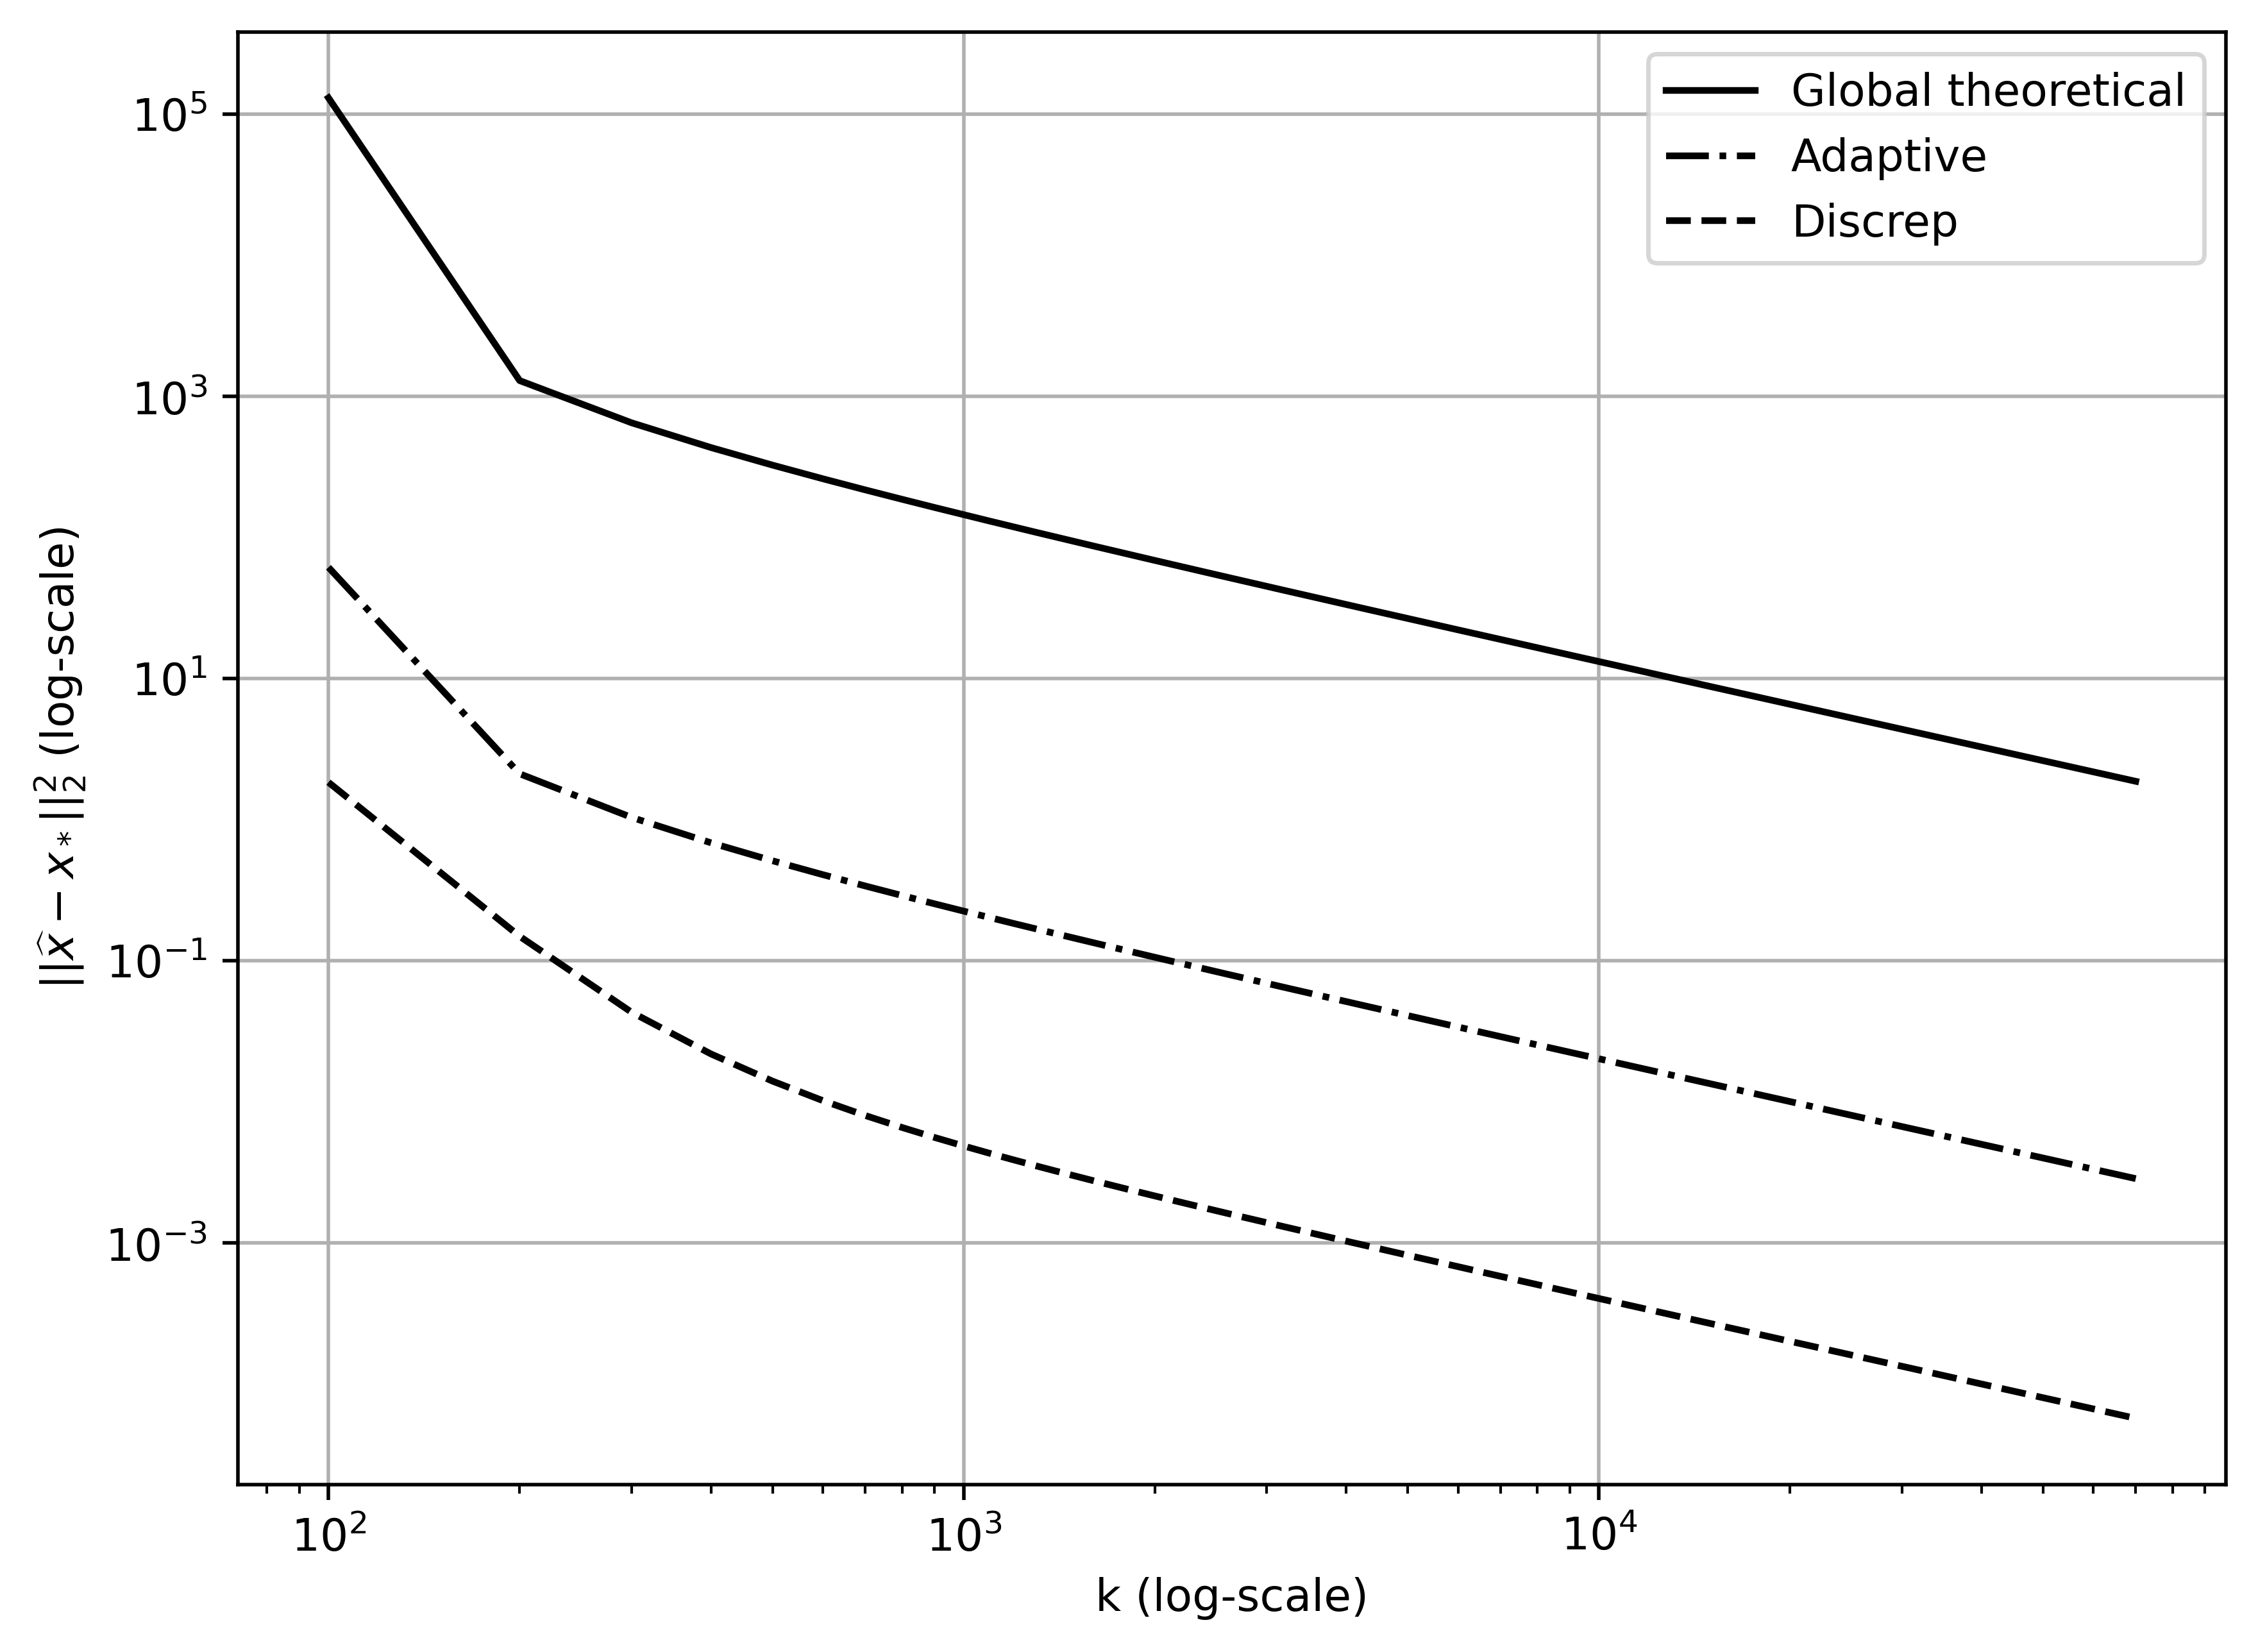
\includegraphics[width=\linewidth]{x_discr_rad_5_q_4_it_70_000_dim_1000.png}
        \endminipage\hfill
        \minipage{0.49\textwidth}
        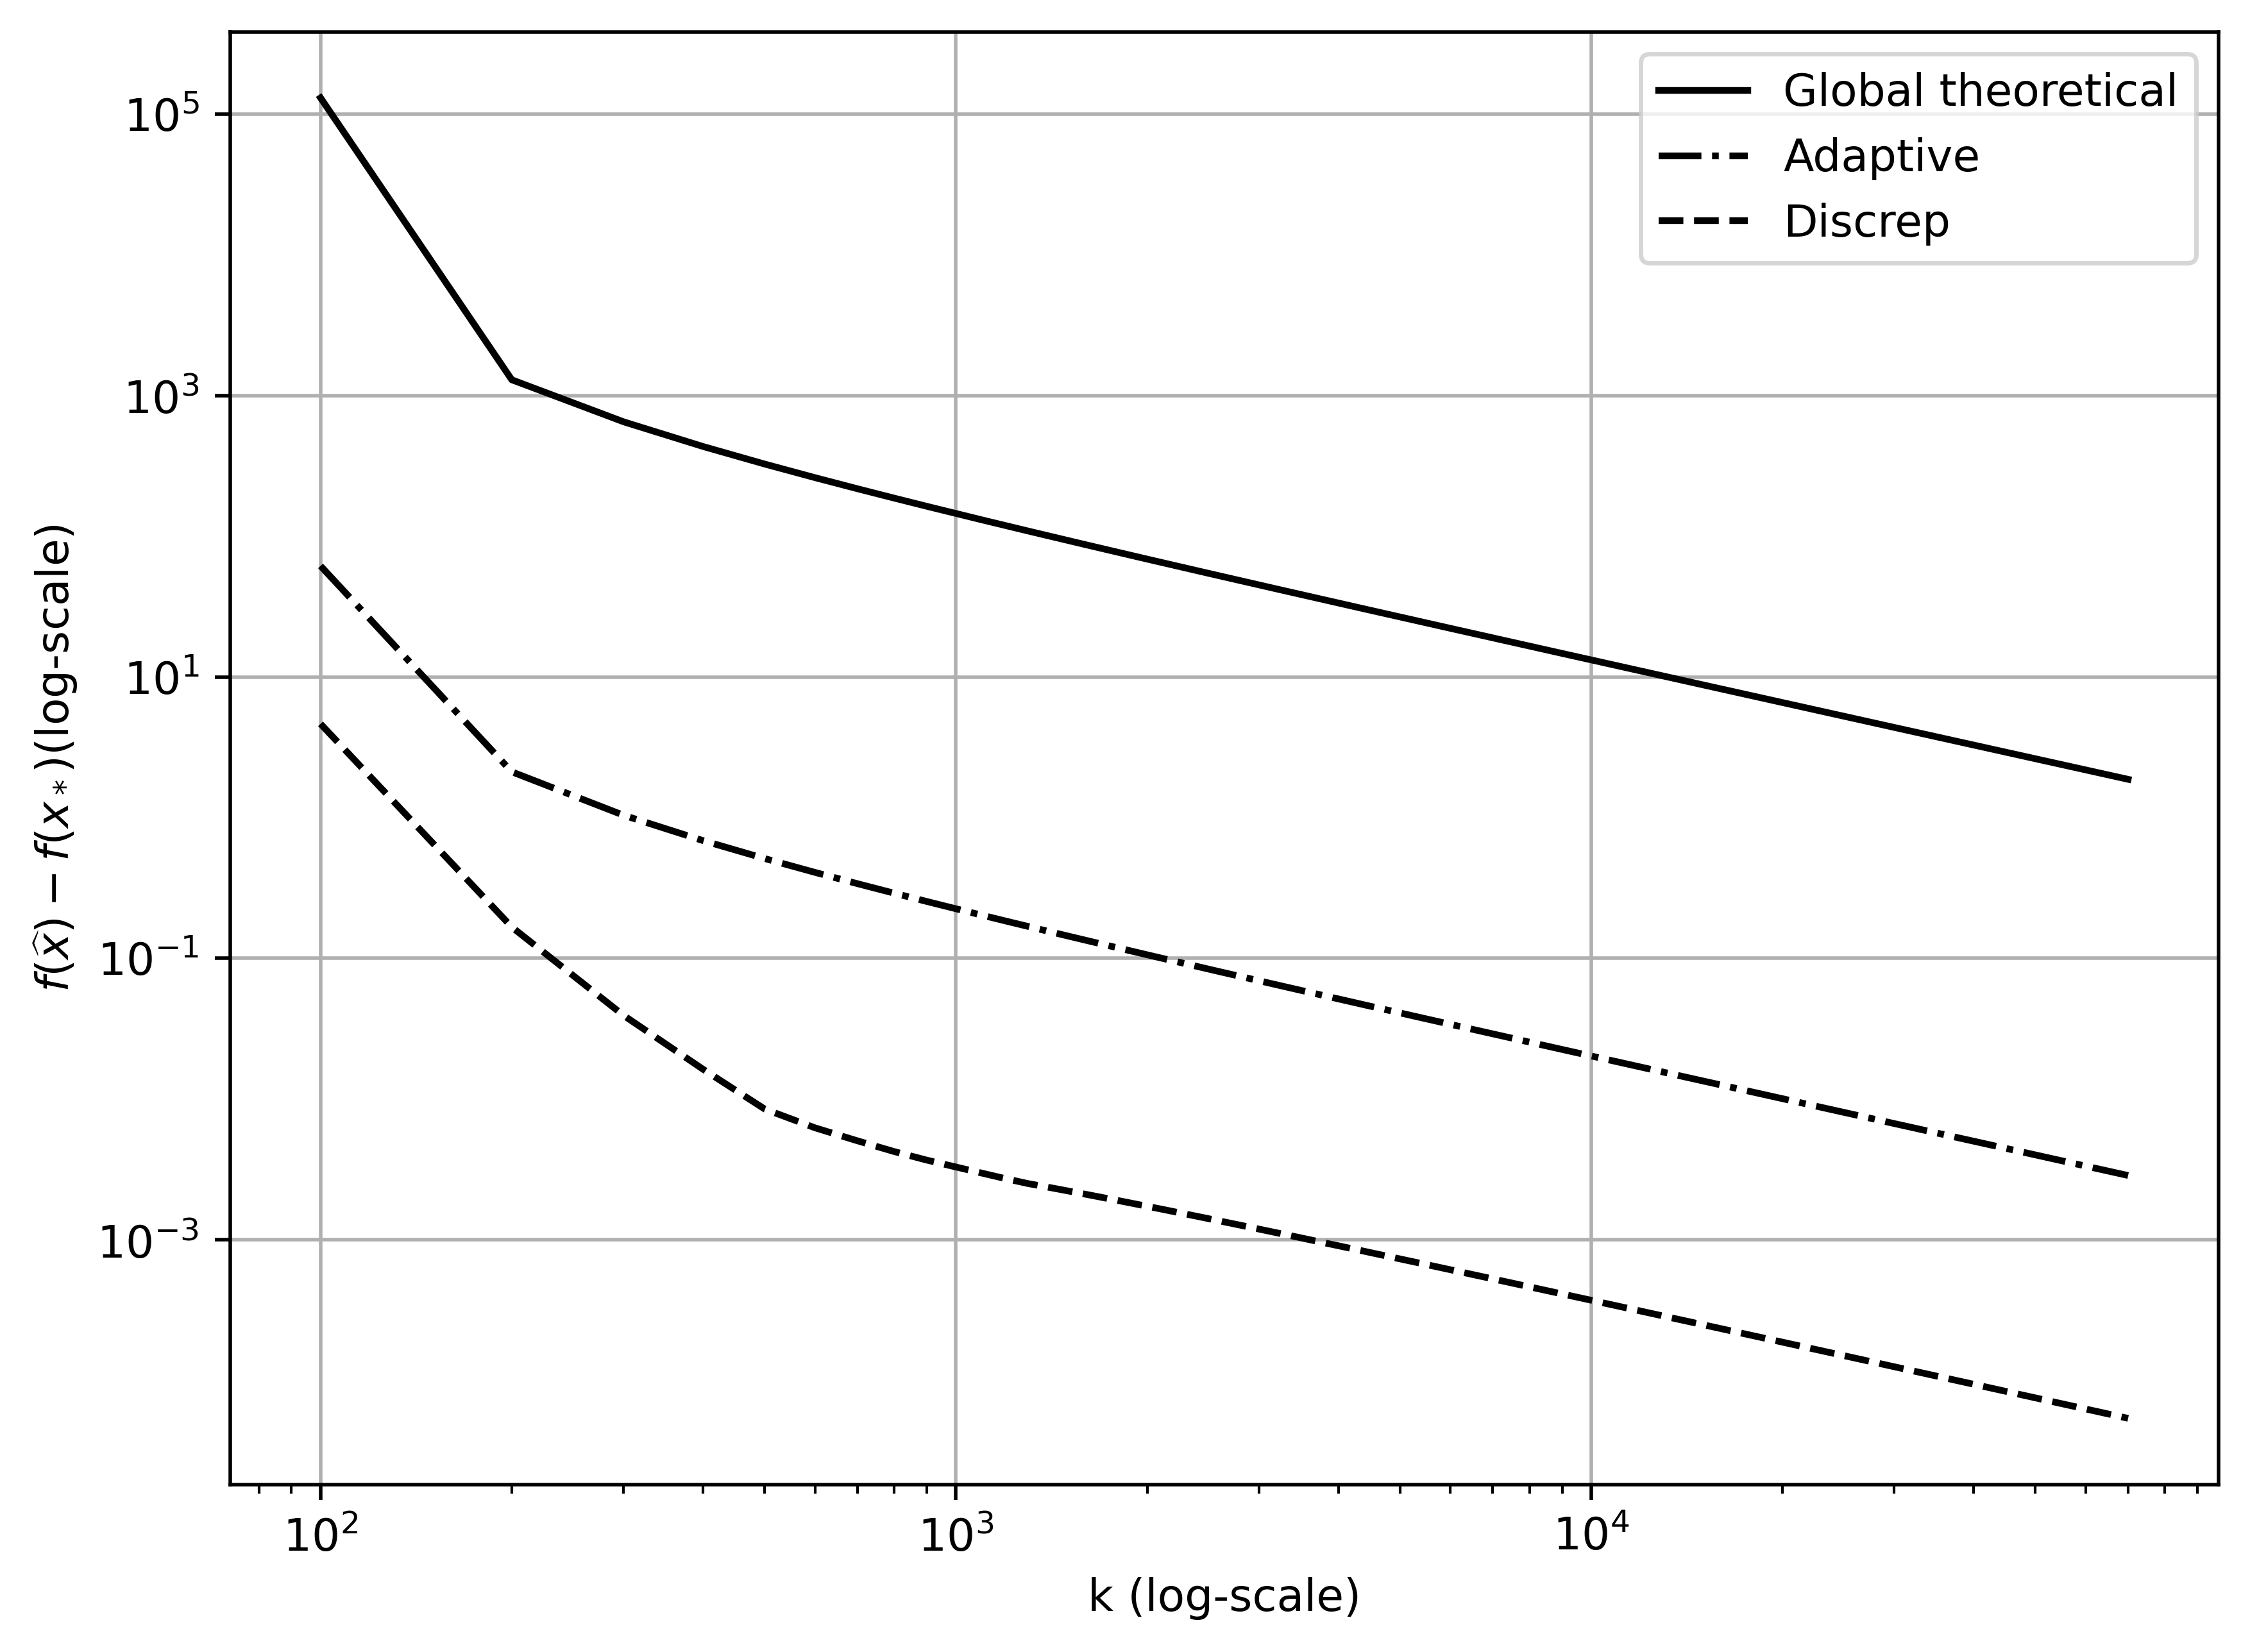
\includegraphics[width=\linewidth]{f_discr_rad_5_q_4_it_70_000_dim_1000.png}
        \endminipage\hfill
        \caption{Результаты решения задачи минимизации \eqref{sphere_cover_strongly}, где  $n= 1\,000, r = 5$ и  шар $Q$ радиуса 4.}
        \label{res_ex_strong_r5}
    \end{figure}

    \begin{figure}[h]
        \minipage{0.49\textwidth}
        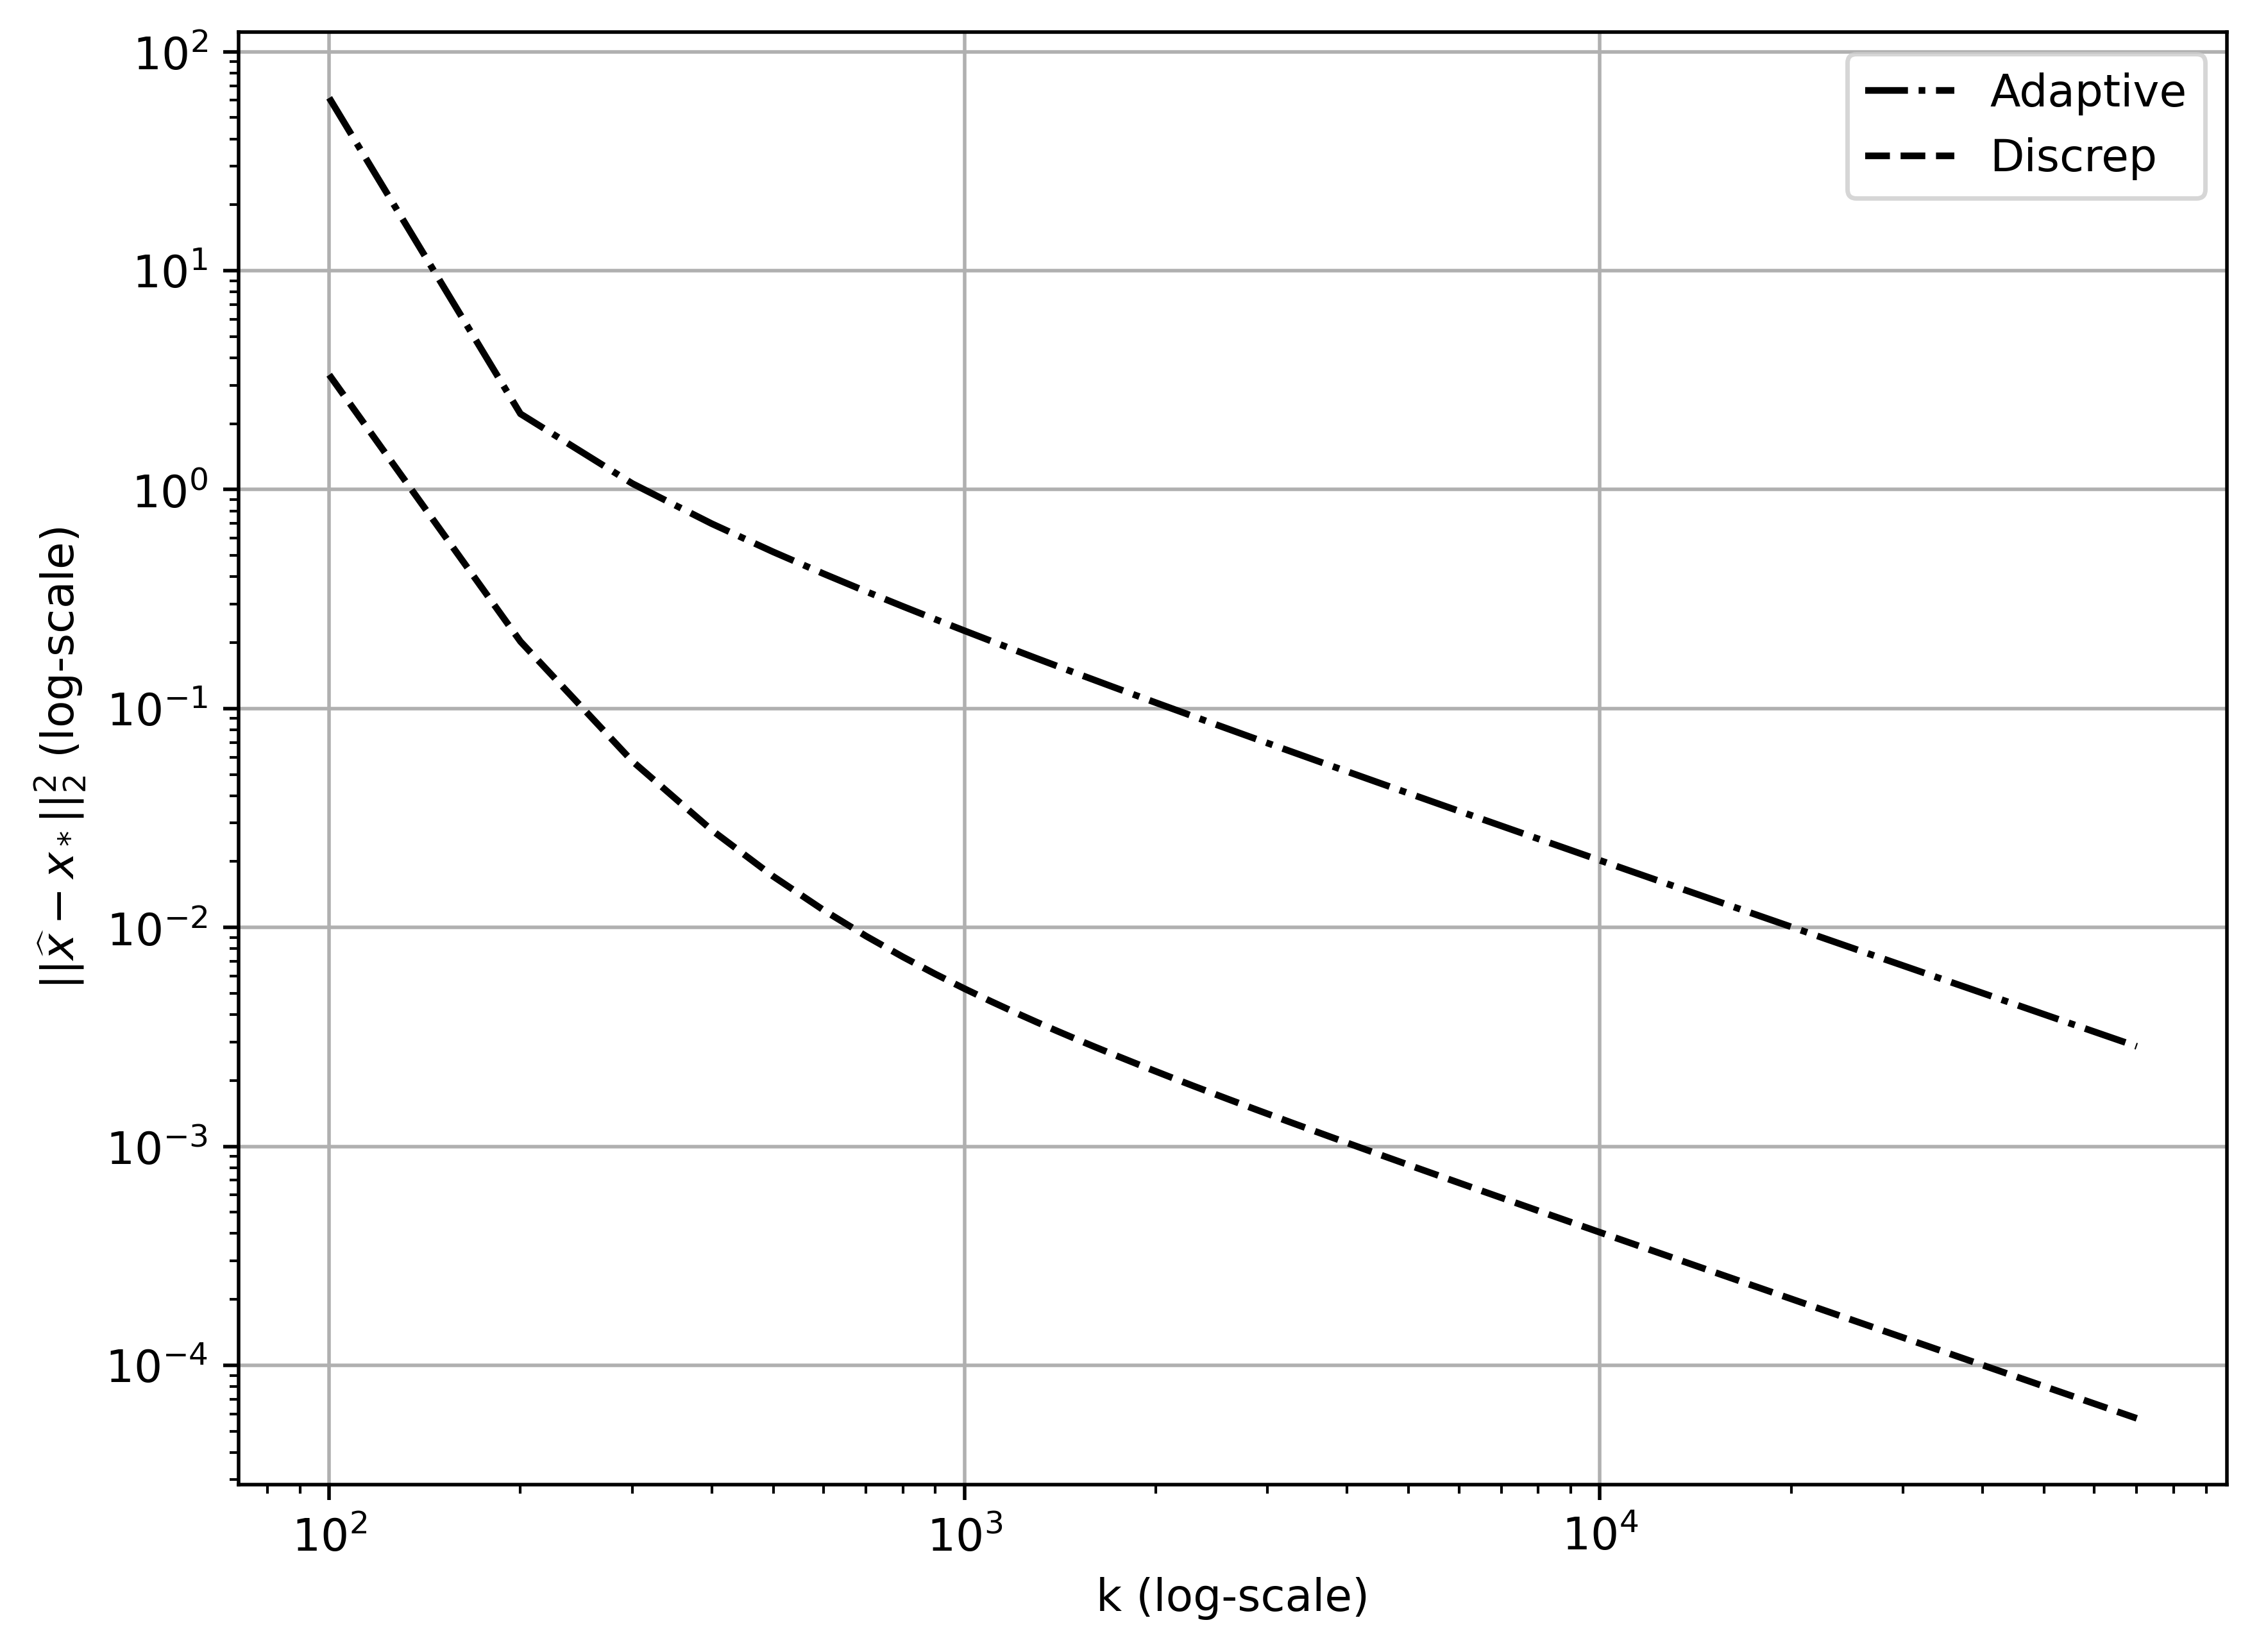
\includegraphics[width=\linewidth]{x_discr_unlim_q.png}
        \endminipage\hfill
        \minipage{0.49\textwidth}
        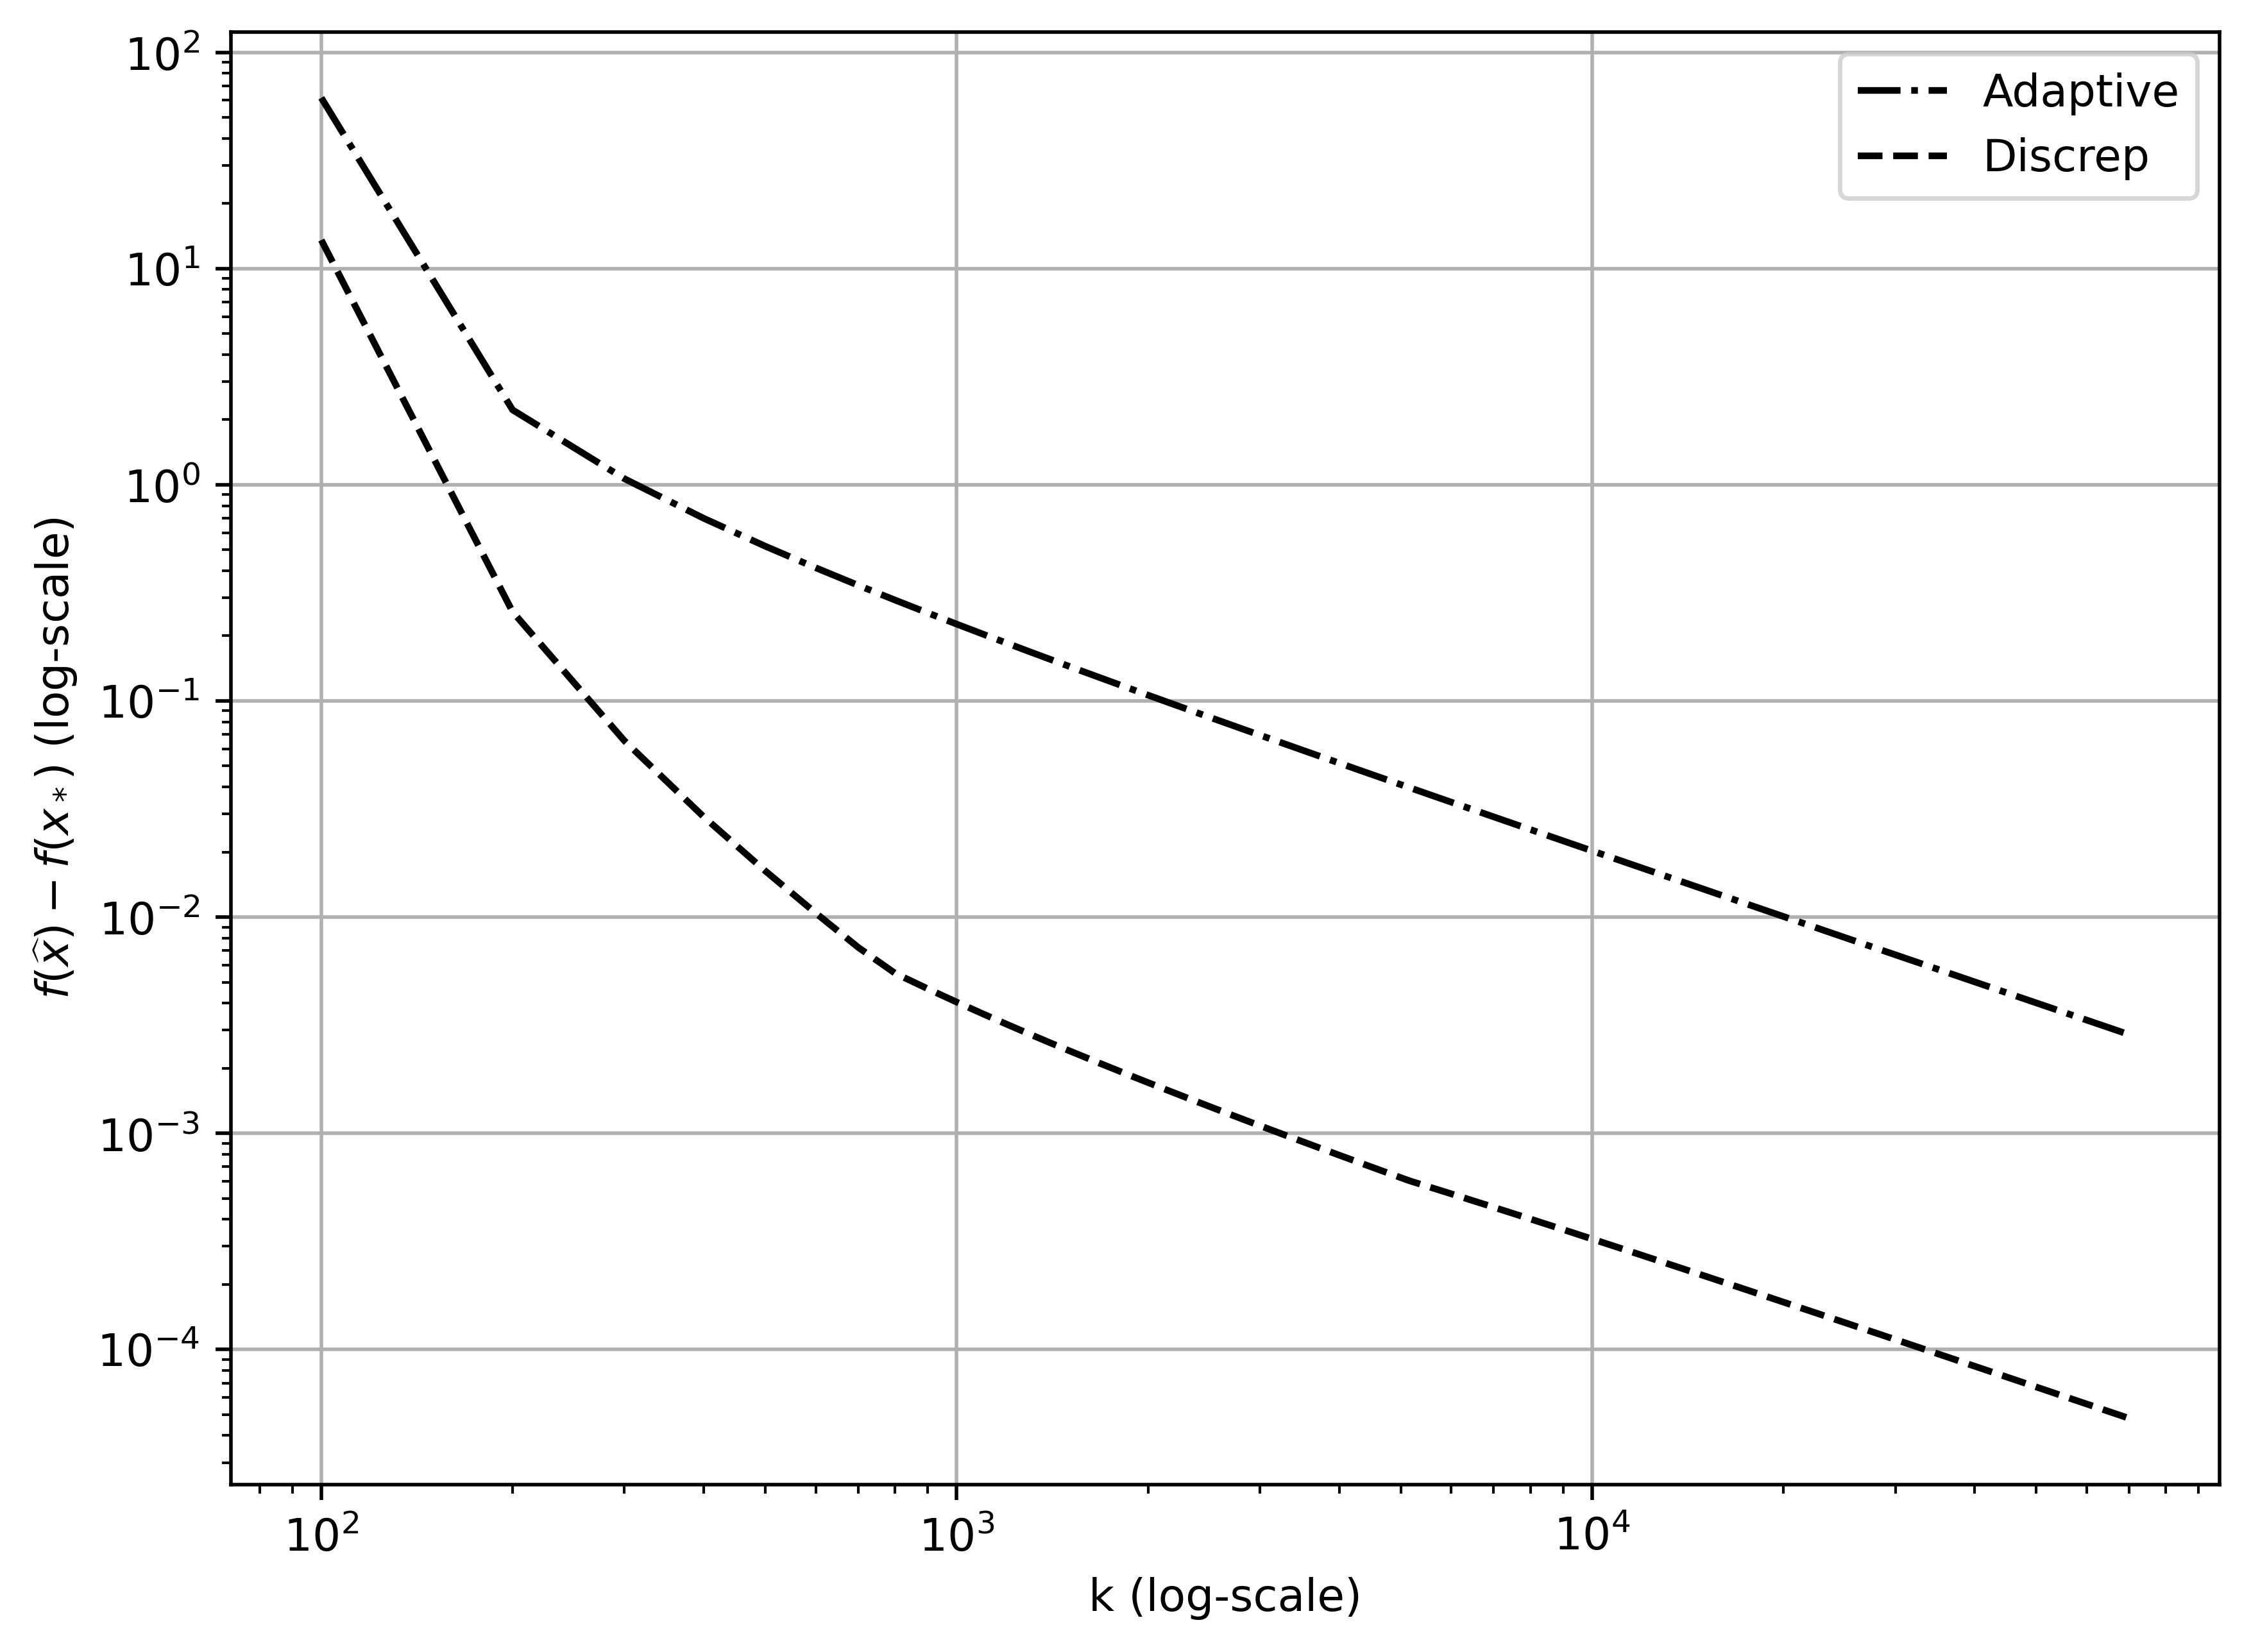
\includegraphics[width=\linewidth]{f_discr_unlim_q.png}
        \endminipage\hfill
        \caption{ Результаты решения задачи минимизации \ref{sphere_cover_strongly}, где  $n= 1\,000, r = 5$ и  $Q = \mathbb{R}^n$.}
        \label{res_ex_strong_unlim}
    \end{figure}

    Теперь перейдём к выпуклой постановке \eqref{sphere_cover} с целью исследования эффективности предложенных в разделе 3 субградиентных методов с $\Delta$-острым мнимимумом. К существующему набору точек, представленных для покрытия, с известным значением центра добавим дополнительную точку, которая находится вне исходного шара достаточно близко к границе (удалена не более, чем на $\Delta > 0$). Данный подход позволяет оценить <<приближённое>> значение минимума $\overline{f}$, что позволит применить разработанные выше варианты субградиентного метода с $\Delta$-острым минимумом. При этом новое значение минимума останется внутри исходной сферы. Поскольку оптимальное значение функции --- это радиус искомого шара, покрывающего все точки, а $x_*$ всегда будет расположена внутри него, то для всякого $x$ верно неравенство $ f(x) \geq \| x - x_*\|_2$. Рассмотрим целевую функцию вида
    \begin{gather}\label{allpha_sphere_cover}
        f(x) := \alpha \max_{x\in Q}\{\|x - a_0\|_2, \|x - a_1\|_2, ..., \|x - a_m\|_2\}.
    \end{gather}
    Тогда значение $\Delta$ можно оценить  из (\ref{eq_gen_sharp}): 
        $f(x) - \overline{f} \geq \alpha\|x- x_*\|_2 - \Delta, \quad \Delta \geq \overline{f}$.

    Отметим, что данная постановка значительно влияет на величину теоретической оценки качества решения (\ref{adaptive_estimate}) для метода \eqref{1}.
    Наиболее значимый вклад в оценку (\ref{adaptive_estimate}) дает последнее слагаемое $\frac{\Delta^2}{2\|\nabla f(x_k)\|^2_2}$, причём 
    $     \Delta \sim \overline{f} \sim \alpha \|\overline{x}-a\|_2 $ и 
    $     \|\nabla f(x_k)\|_2 = \alpha $. Поэтому последнее слагаемое пропорционально радиусу шара, соответсвующему <<приближённому>> решению. Это и подтверждается экспериментально. Для сравнения, ниже на рис. \ref{res_sharp_convex} и \ref{res_strong_convex} приведены результаты работы для того же набора входных точек, которые необходимо покрыть в обоих постановках --- (\ref{allpha_sphere_cover}) и (\ref{sphere_cover_strongly}). Начальная точка также одна и та же. Сравниваются методы \eqref{1} и \eqref{orig}. Первый из этих методов обеспечивает сходимость буквально за 10 итераций к <<приближённому>> решению с заданной точностью и даже позволяет эту точность повысить. Второй же метод достигает схожих (с геометрической точки зрения) результатов за значительно большее количество итераций, однако он позволяет повышать точность приближённого решения на дальнейших итерациях.

    Подтверждение данного теоретического наблюдения хорошо иллюстрируется на рис. \ref{res_sharp_convex} и \ref{res_strong_convex}. На рис. \ref{res_sharp_convex} показано поведение субградиентного спуска, использующего $\Delta$-острый минимум (теорема \ref{theorem4}), а именно --- быстрая сходимость к <<приближенному>> решению. Штрих-пунктирная линия соответствует оценке \eqref{eq_gen_sharp}, а штриховая --- невязке по функции и аргументу. На рис. \ref{res_strong_convex} показано поведение метода для той же задачи, но с использованием сильно выпуклого целевого функционала (теорема \ref{ThmBachAdaptive}). Скорость убывания уже не столь высокая, но точность получаемого решения в итоге выше. Сплошная линия --- это глобальная оценка \eqref{orig_estimation_f}, штрих-пунктирная --- адаптивная \eqref{adaptive_estimation_f}, а штриховая --- невязка по функции и аргументу.

    \begin{figure}[h]
        \minipage{0.49\textwidth}
        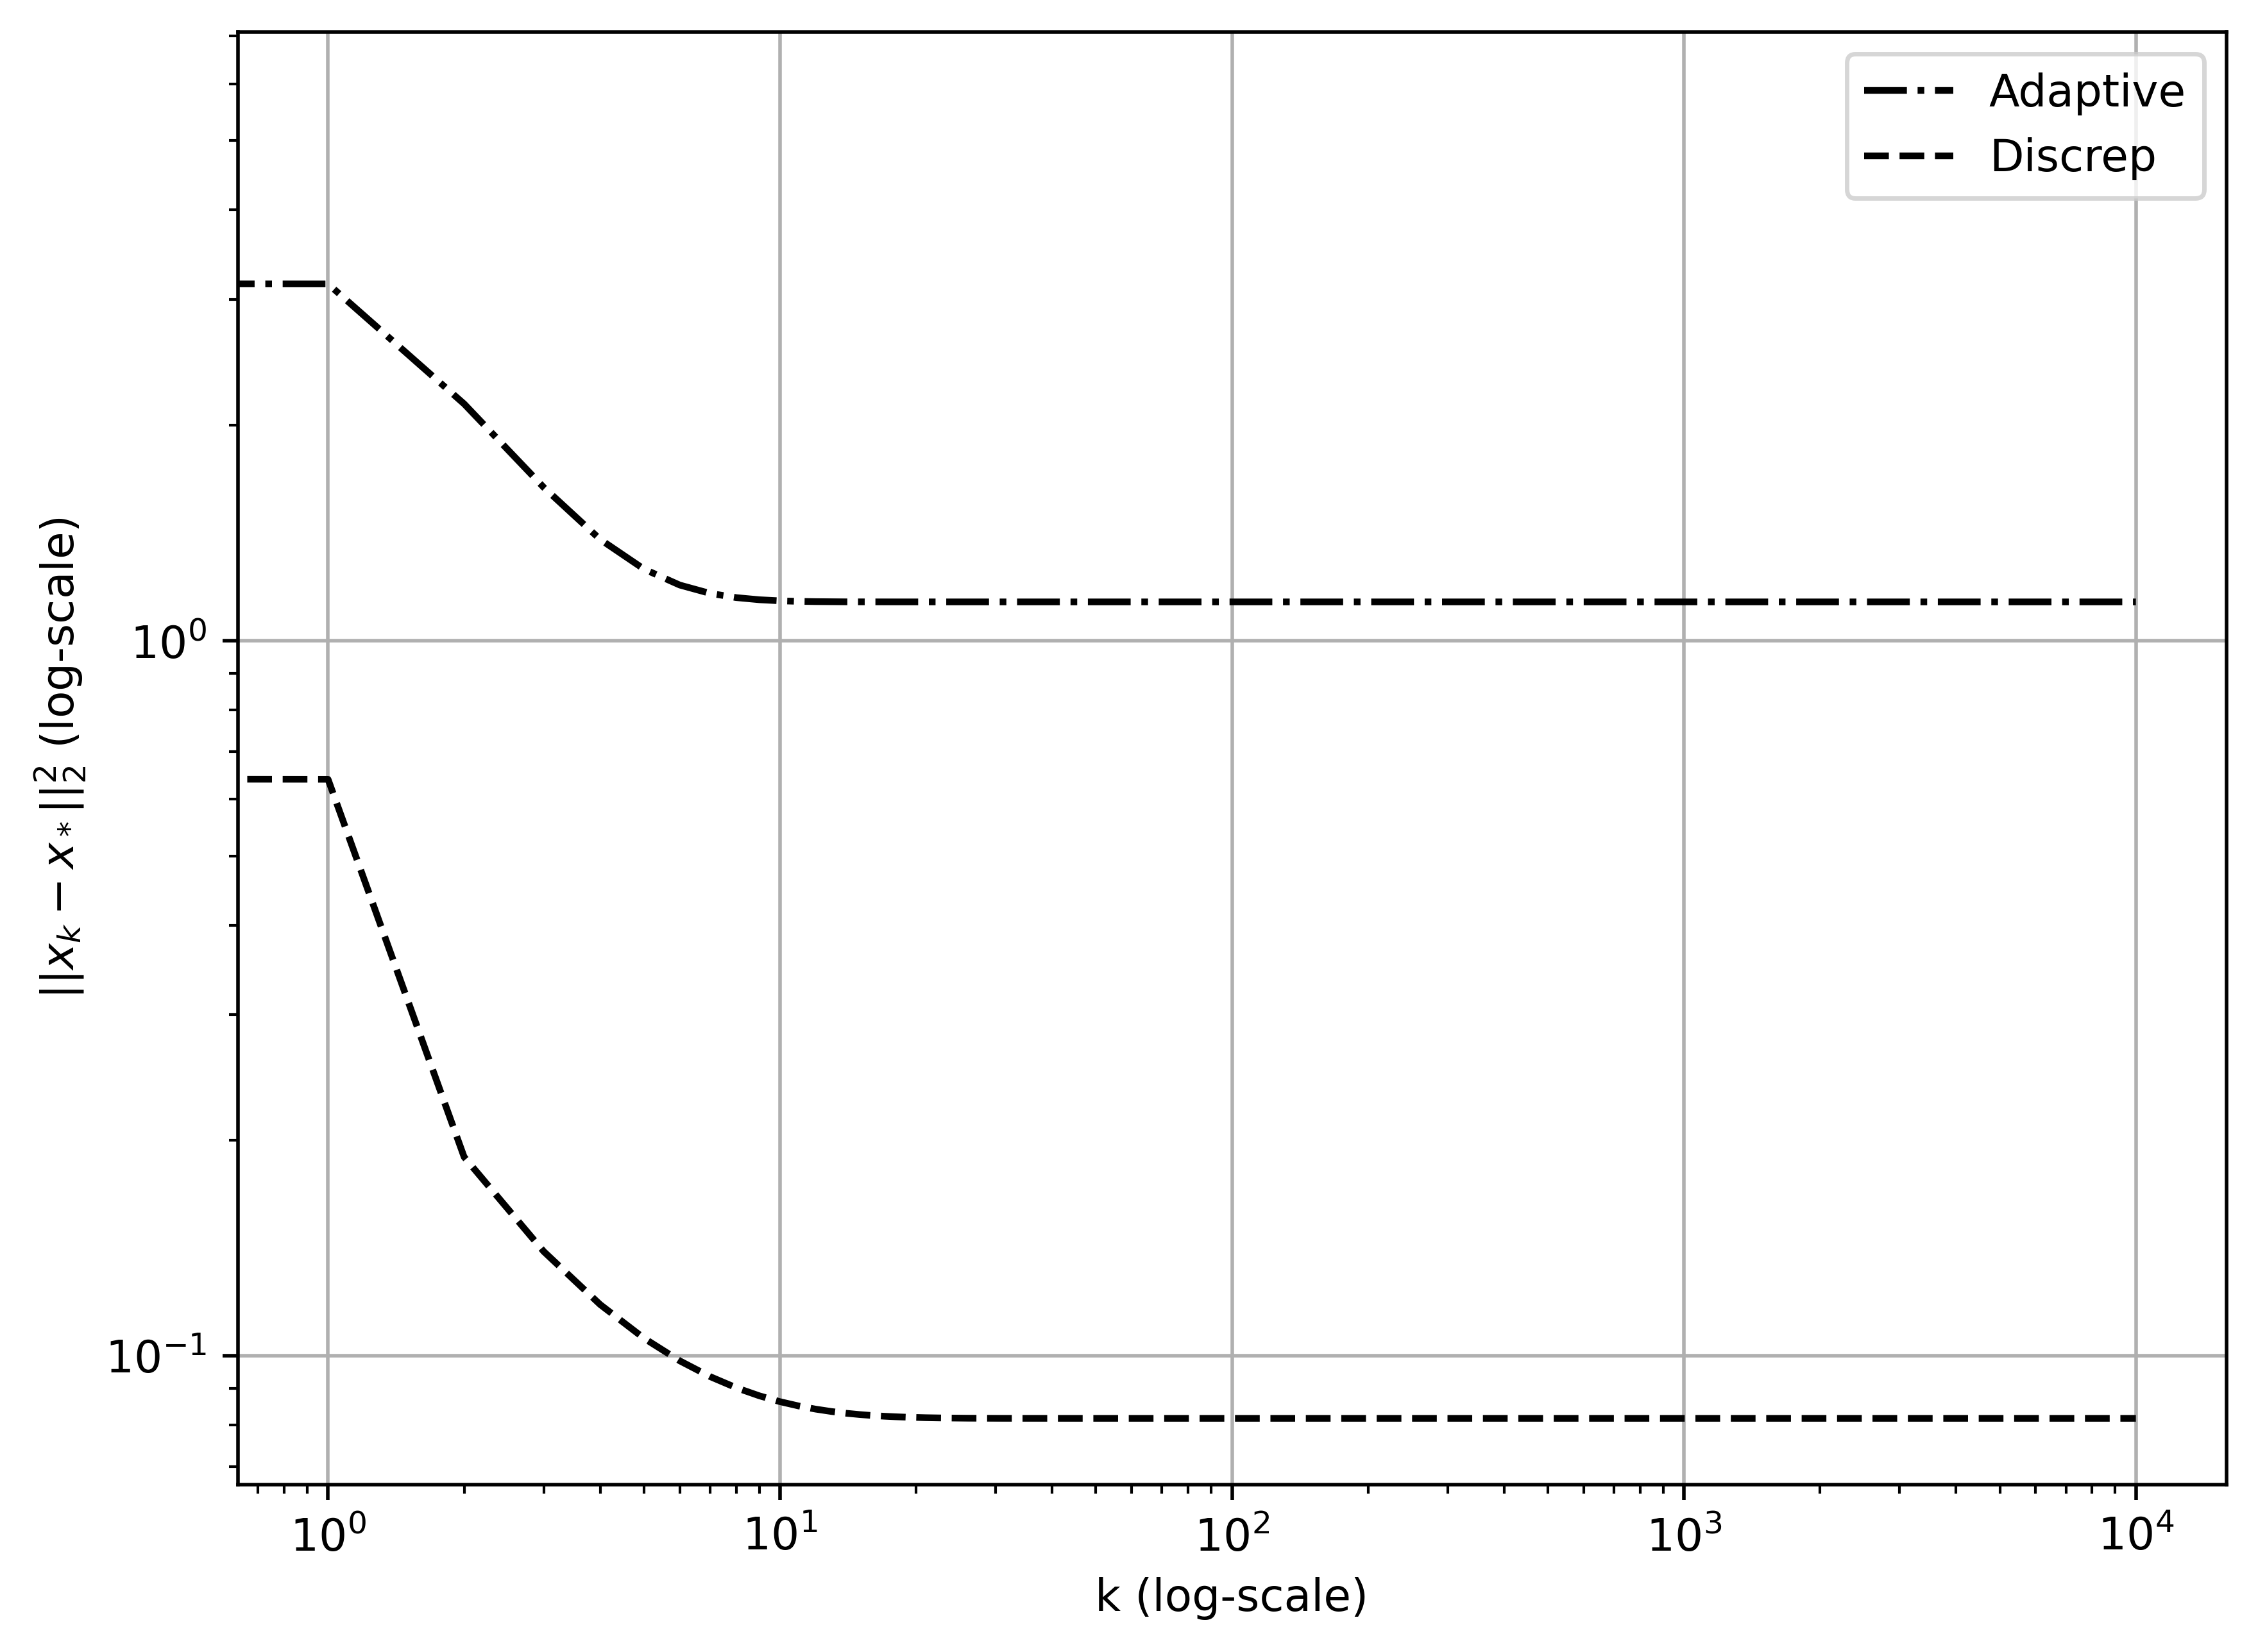
\includegraphics[width=\linewidth]{sharp_convex_x.png}
        \endminipage\hfill
        \minipage{0.49\textwidth}
        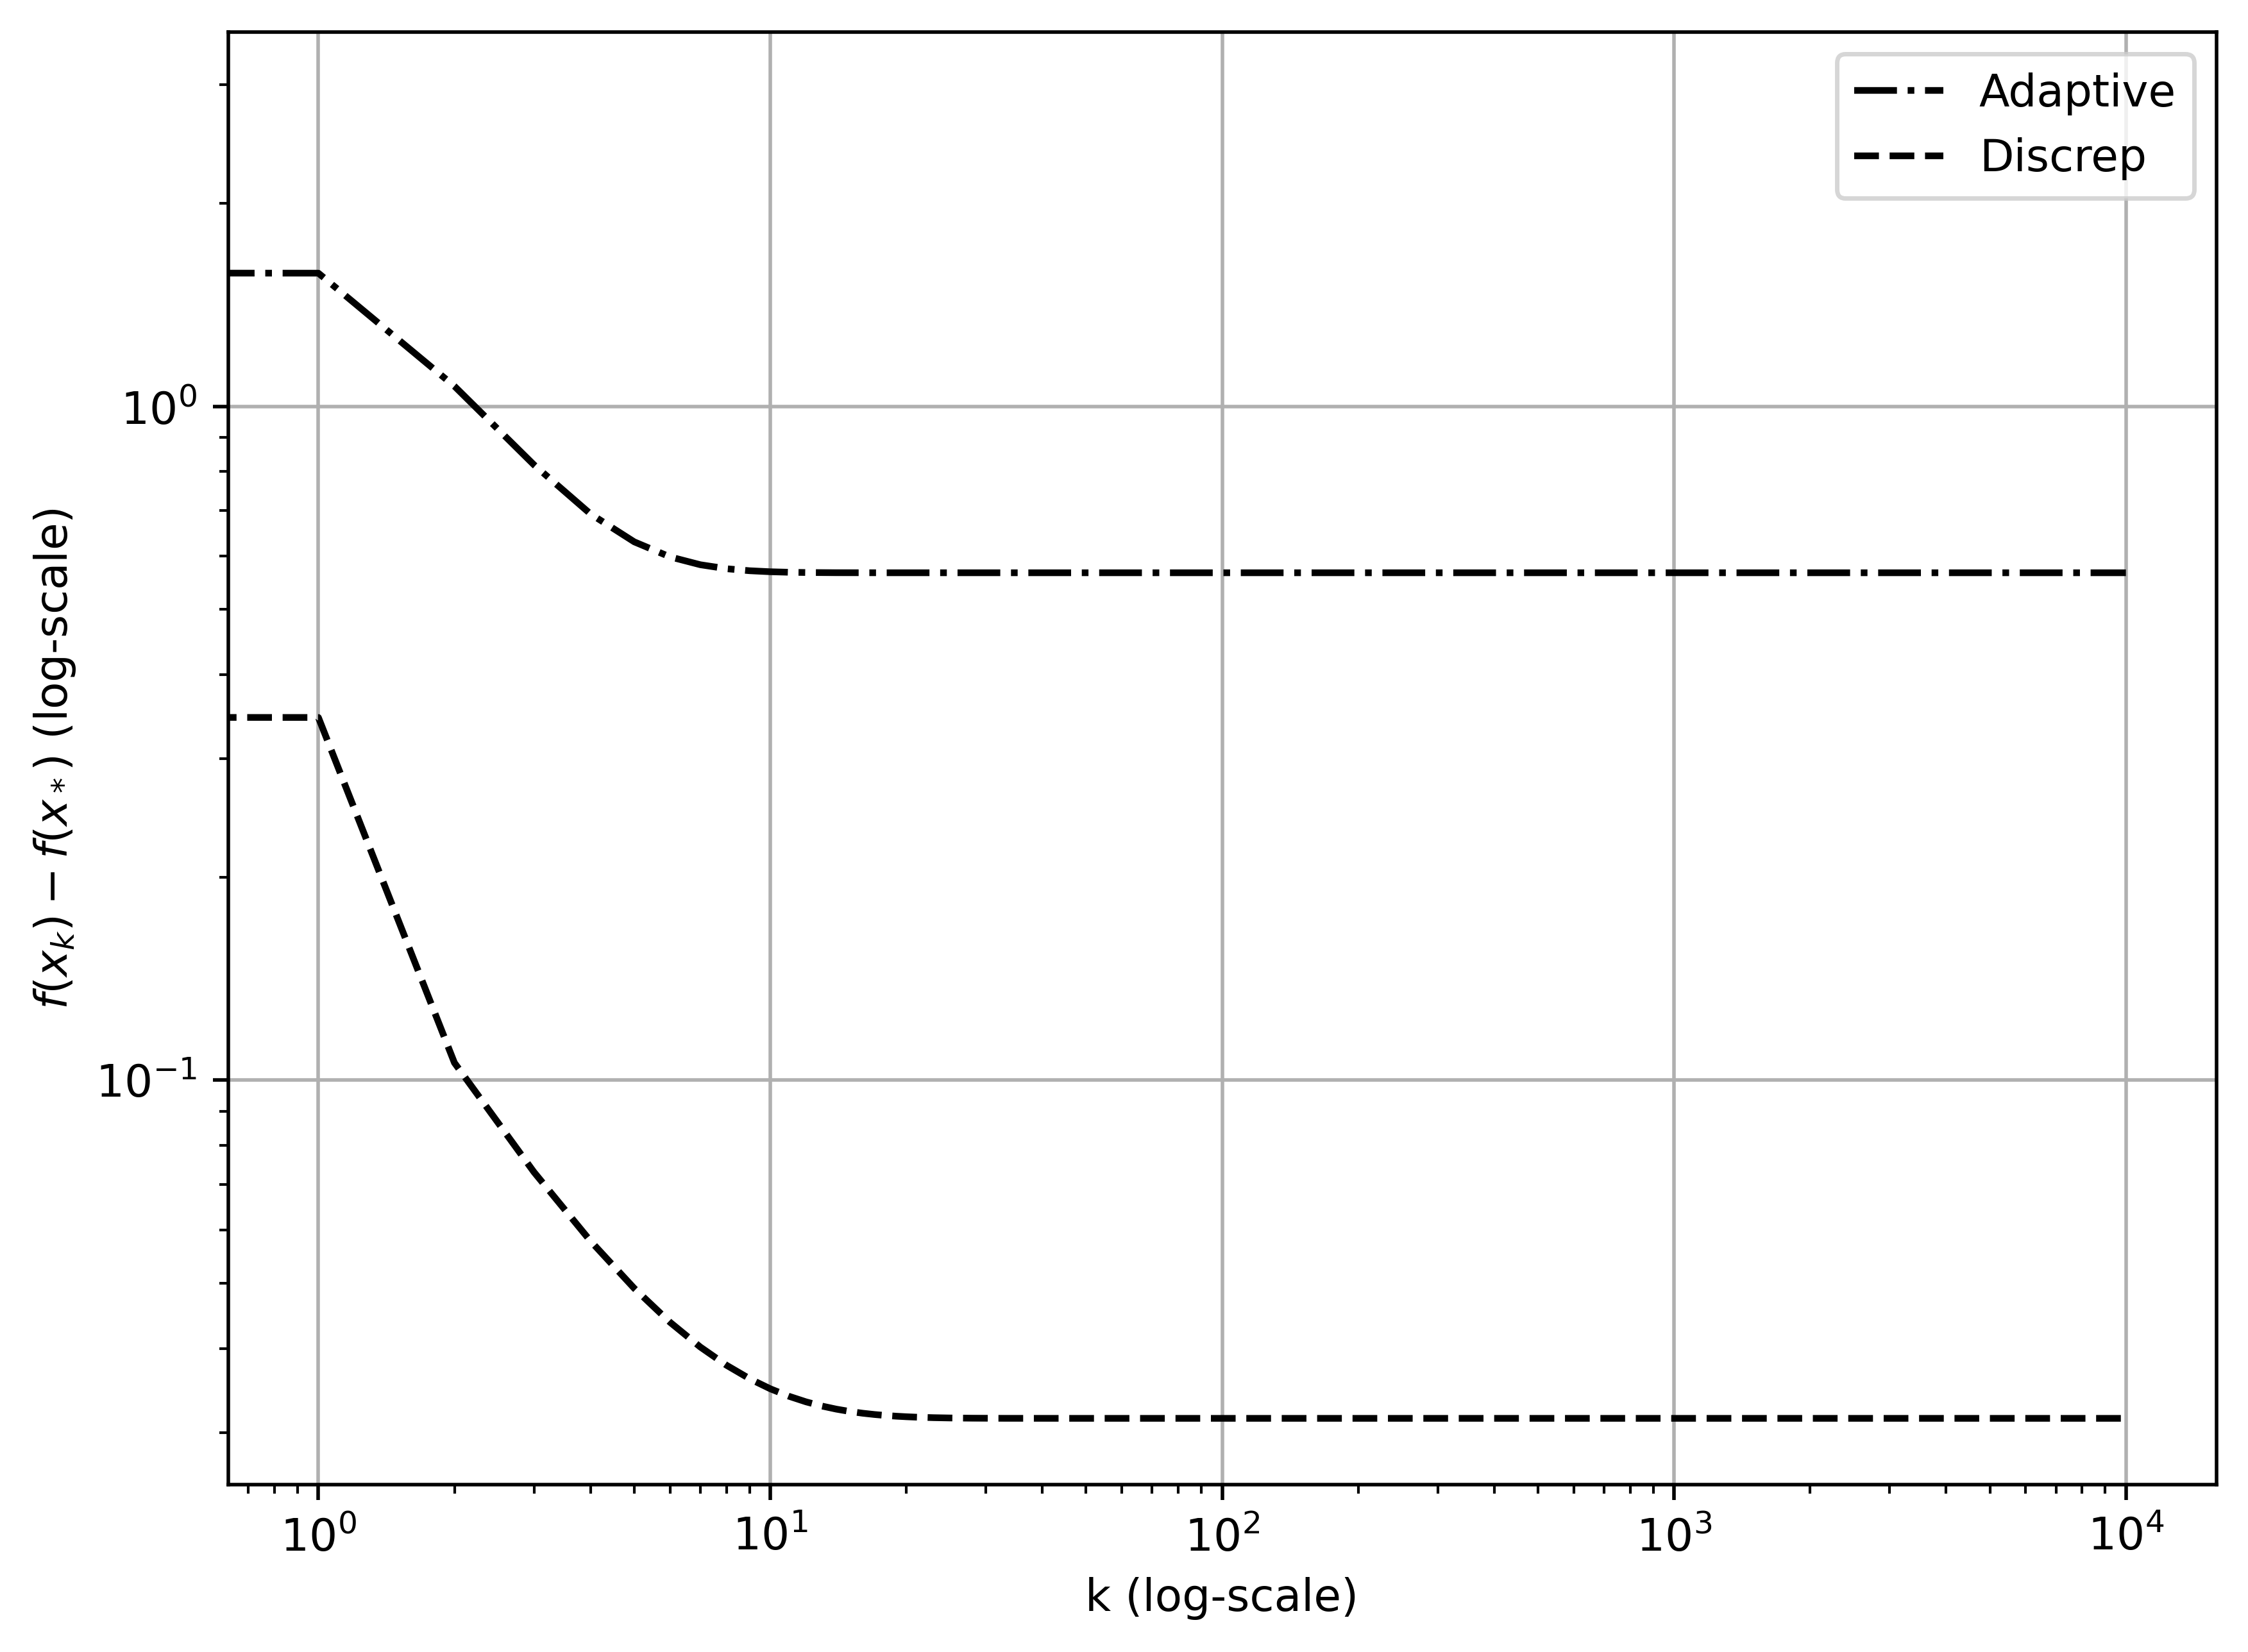
\includegraphics[width=\linewidth]{sharp_convex_f.png}
        \endminipage\hfill
        \caption{ Результаты решения задачи минимизации (\ref{allpha_sphere_cover}), где  $n= 1\,000, r = 0.7525, \alpha = 0.6$.}
        \label{res_sharp_convex}
    \end{figure}

    \begin{figure}[h]
        \minipage{0.49\textwidth}
        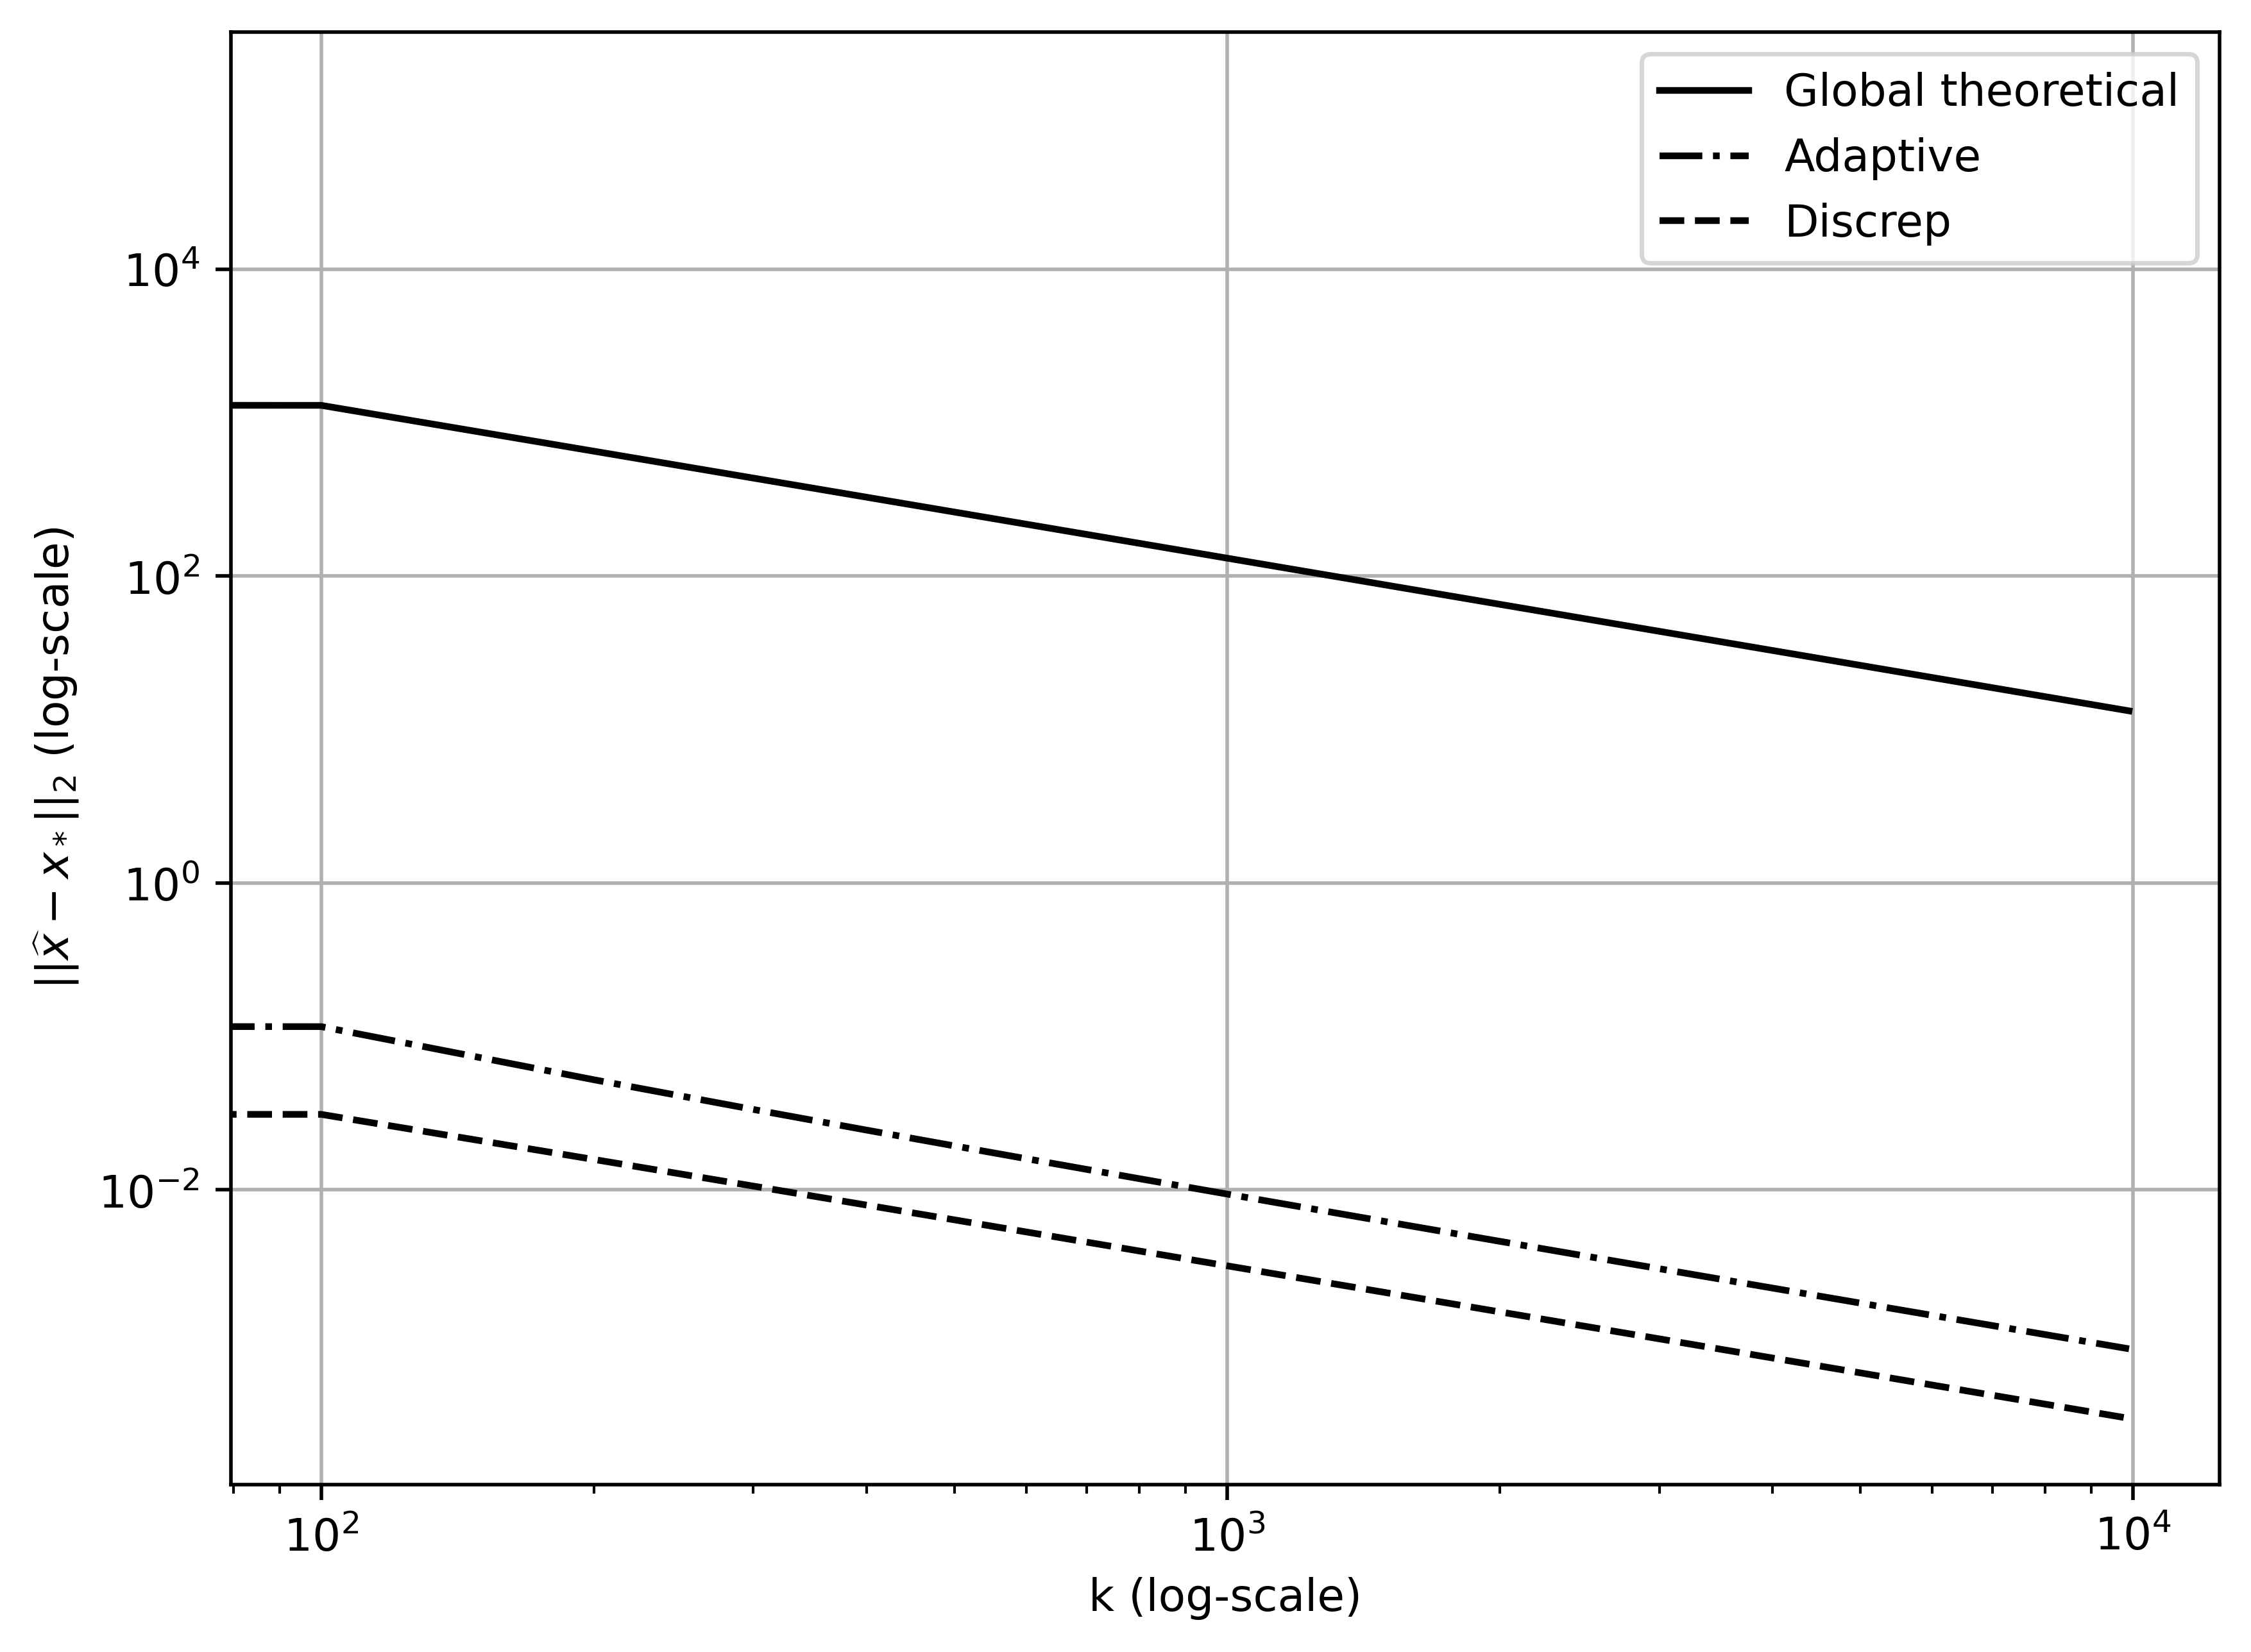
\includegraphics[width=\linewidth]{strong_convex_small_rad_x.png}
        \endminipage\hfill
        \minipage{0.49\textwidth}
        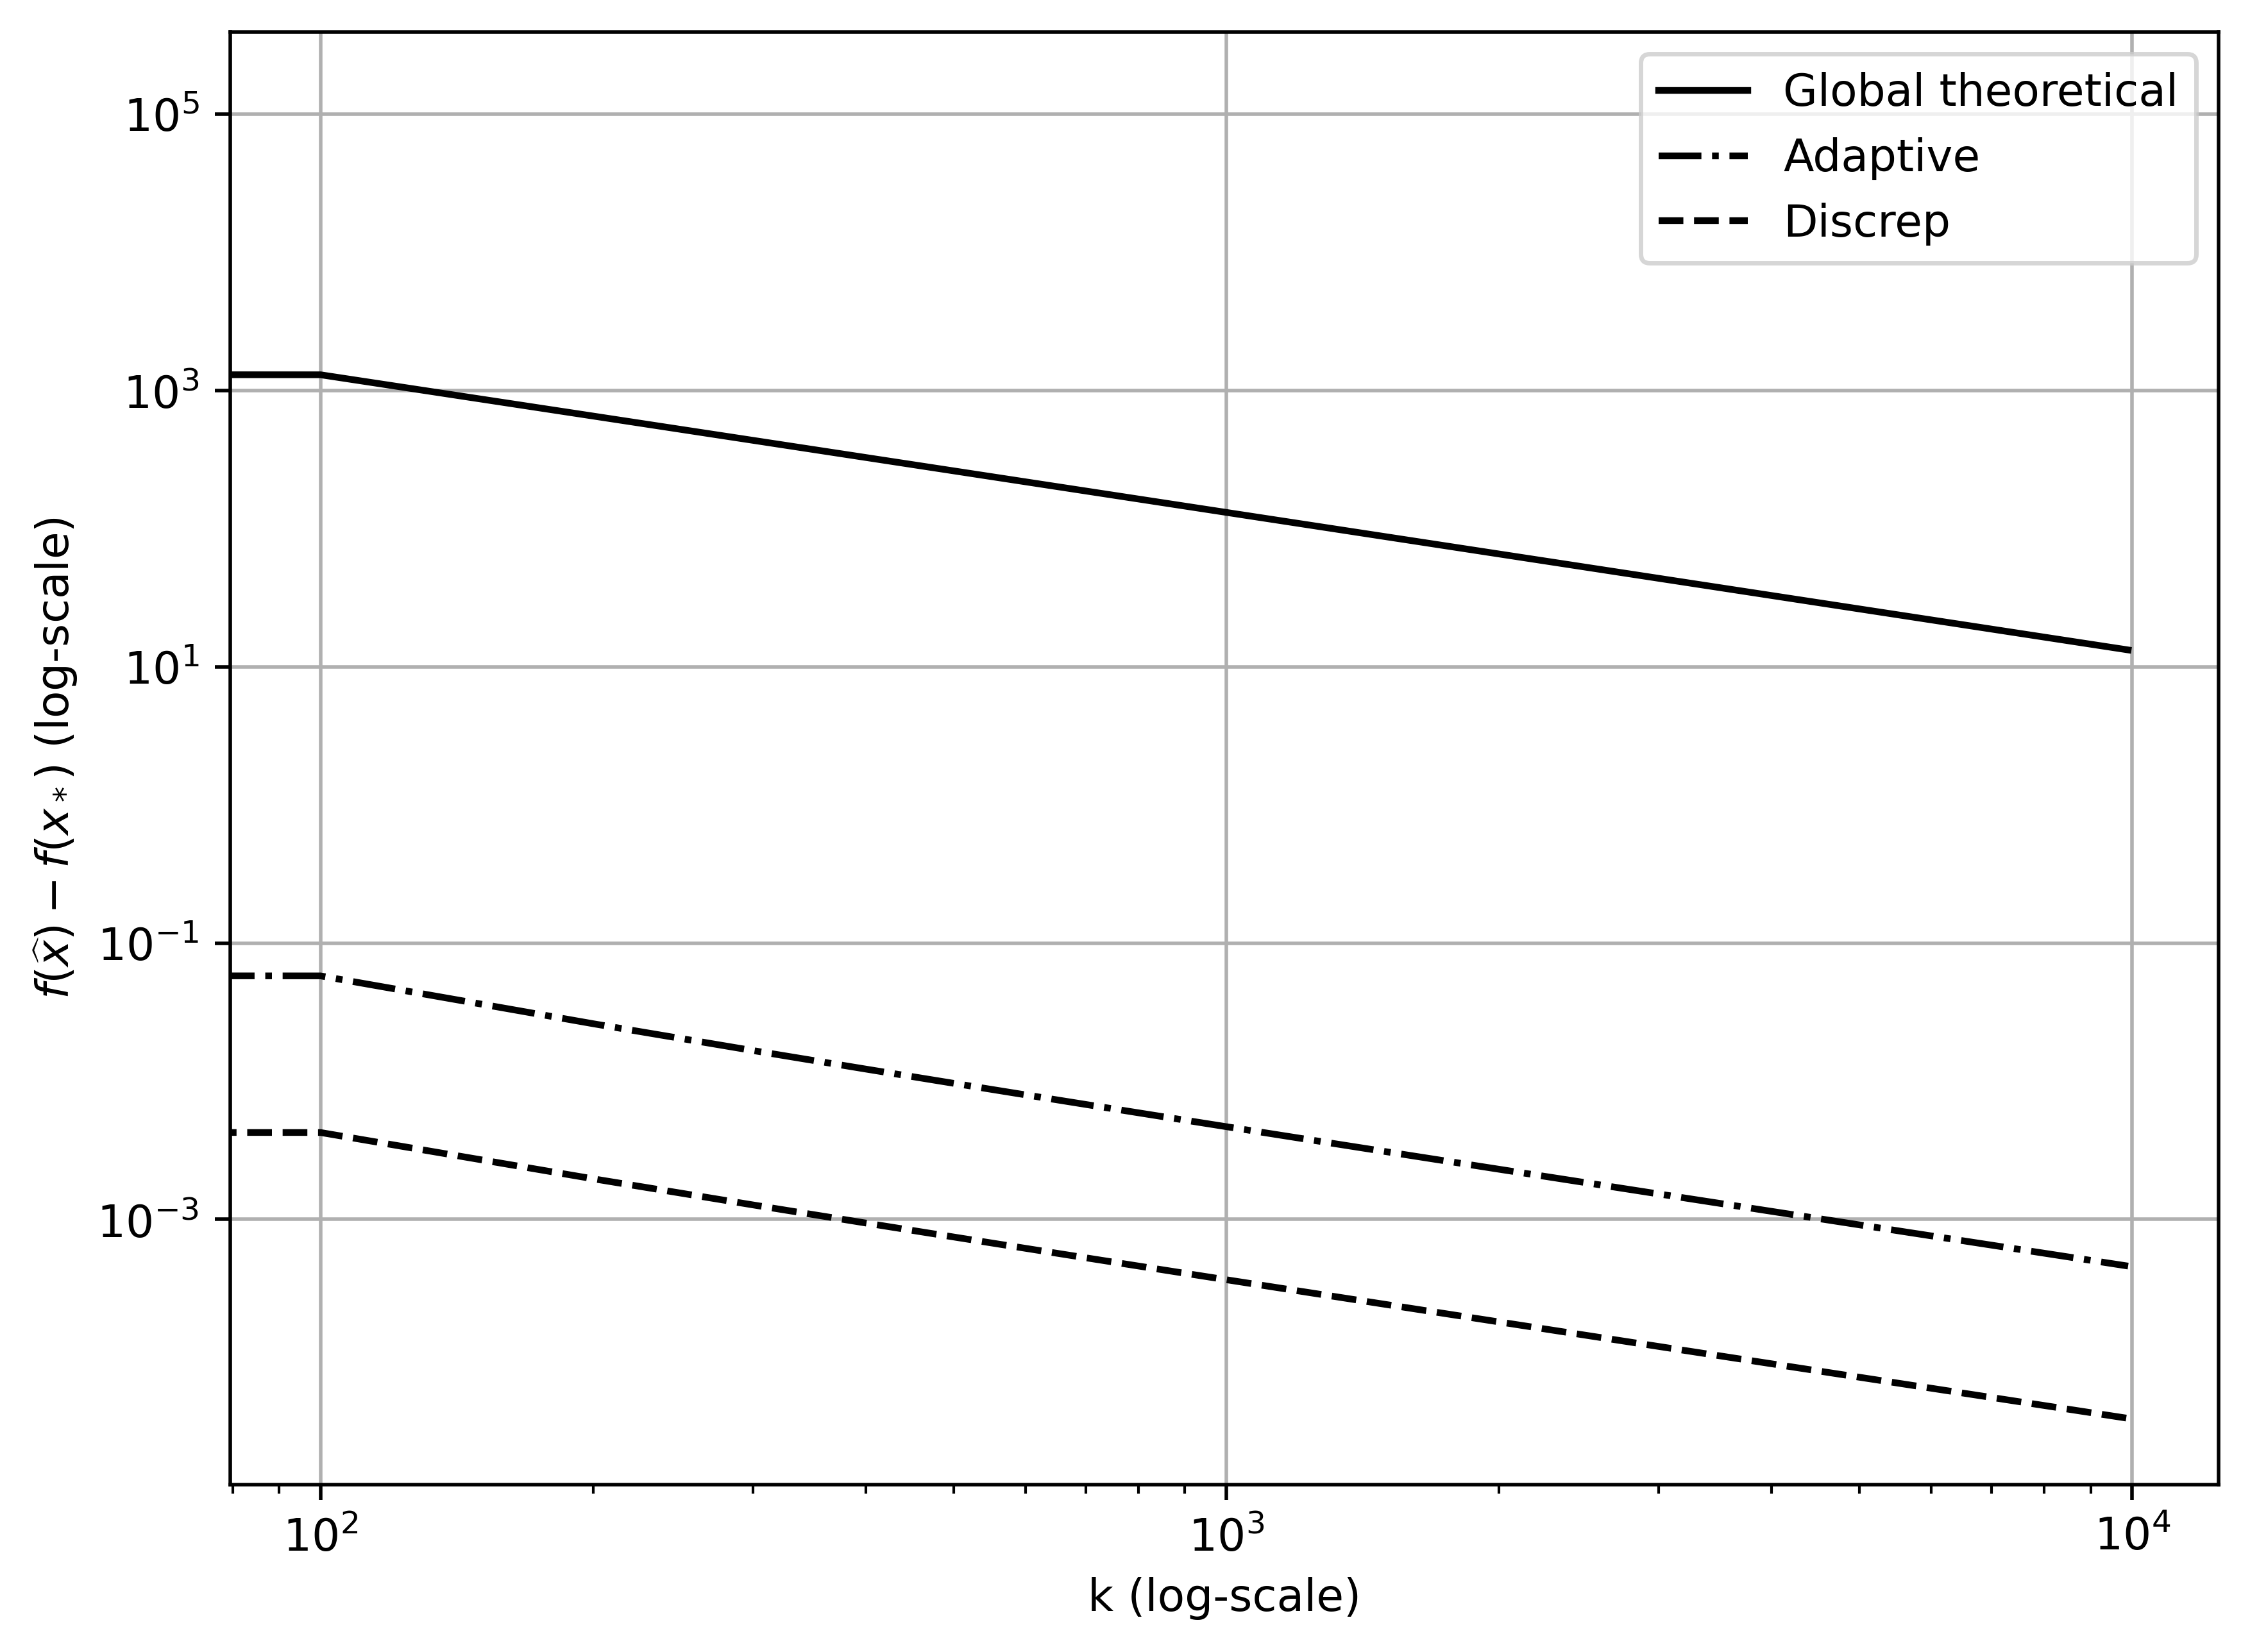
\includegraphics[width=\linewidth]{strong_convex_small_rad_f.png}
        \endminipage\hfill
        \caption{ Результаты решения задачи минимизации (\ref{sphere_cover_strongly}), где  $n= 1\,000, r = 0.7525$.}
        \label{res_strong_convex}
    \end{figure}

    Тем не менее, сравнение с известным точным решением $x_*$, а также график динамики значения целевой функции показывает, что за малое число шагов (значительно меньшее, чем для метода \eqref{orig}) реализация метода \eqref{1} приводит к неплохому качеству приближённого решения. При этом, однако, для метода \eqref{1} после достижения такого уровня дальнейшее повышение качества выходной точки в отличие от метода \eqref{orig} уже не наблюдается.

\FloatBarrier